%!TEX root = ../thesis.tex
%*******************************************************************************
%*********************************** Signal region optimisation *********
%*******************************************************************************


\chapter{Signal region optimisation}

\ifpdf
    \graphicspath{{chapter-optimisation/Figs/Raster/}{chapter-optimisation/Figs/PDF/}{chapter-optimisation/Figs/}}
\else
    \graphicspath{{chapter-optimisation/Figs/Vector/}{chapter-optimisation/Figs/}}
\fi

\glsreset{sr}

In order to discover the rare signals predicted by the \gls{susy} models considered, dedicated kinematic regions enriched in signal events, so called \gls{sr} are constructed. They are optimised to be able to discover a maximum number of the signal models considered in the analysis. In this chapter, the \gls{sr} optimisation procedures leading to the final \glspl{sr} are introduced and discussed. 

\section{Optimisation methods}

All optimisation methods used in the following need a figure of merit that should be maximised in order to define the best performing setup. While the multidimensional cut scan in \cref{sec:n-dim-scan} and the N-1 plots approach in \cref{sec:n-1-scan} use the binomial discovery significance $Z_\mathrm{B}$ introduced in~\cref{sec:sensitivity_estimation}, the fit scan procedure in \cref{sec:fit-scan} aims to maximise the area of the expected exclusion contour.

\subsection{Multidimensional cut scan}\label{sec:n-dim-scan}

The first optimisation method used for designing the \glspl{sr} is an $N$-dimensional cut scan using $N$ observables. For each unique combination of requirements on the set of considered observables, the expected signal and background rate as well as the statistical uncertainty on the background rate is determined from the \gls{mc} samples. As this takes a non-negligible amount of time, it is crucial to restrict the amount of cut combinations. By comparing with distributions at preselection level as \eg shown in \cref{fig:norm_obs}, a set of discrete cuts can be defined for each observable. In practice, a total number of $\mathcal{O}(10^7-10^8)$ cut combinations can still be tested on a single machine with a reasonable turnaround time. 

After determining the excepted event rates and statistical uncertainties, the different cut combinations are binned into a predefined number of signal efficiency bins. For each bin, the background rejection is subsequently maximised, \ie the cut combination with the highest background is chosen as a candidate combination for the respective signal efficiency bin. Cut combination candidates maximising the background rejection are assumed to also maximise the discovery significance. With the significance definition used herein, this is in general a valid assumption is it tends to monotonically increase with decreasing background rate, even when the statistical uncertainty on the background estimation increases due to tighter requirements and less available \gls{mc} statistics. This procedure effectively generates a \gls{roc} curve. As only a small subset of all tested cut combinations are selected as candidates and lie on the \gls{roc} curve, more computationally intensive calculations can be performed, as \eg calculating the discovery significance. This is illustrated in a small scan using $10^4$ cut combinations in \cref{fig:ahoi_examples}. 

A common problem of $N$-dimensional scans is the concept of \textit{overtightening} the selections given the available \gls{mc} statistics. Since the cross sections of the considered \gls{susy} process are many orders of magnitude smaller than those of most of the \gls{sm} processes, it is necessary to apply tight requirements on the kinematic observables in order to achieve a significant signal-to-background separation. However, due to the finite amount of \gls{mc} statistics available, many of the more extreme cut combinations select kinematic regions where not enough \gls{mc} statistics are available for a reasonable estimation of the background rates. Thus, by maximising the background rejection, it may occur that cut combinations are selected where the mere lack of \gls{mc} statistics to properly estimate the background rates causes a high significance value. As the significance values obtained for such configurations are naturally not trustworthy, they need to be avoided. 

In the $N$-dimensional cut scan implementation used herein, the available \gls{mc} datasets are split in two statistically independent, equally sized subsets. This allows to compute two independent values for the discovery significance for each cut combination candidate, as well as having two \gls{roc} curves for each scan. A large difference in either the significance values or the \gls{roc} curves then is a clear indication that too tight cuts are applied for the available \gls{mc} statistics. In addition, requirements on the minimum number of raw \gls{mc} events for different background processes, as well as the maximum allowed statistical uncertainty on a given process, are applied. In the following, the $N$-dimensional cut scan implementation provided by \texttt{ahoi}~\cite{ahoi} is used.

 \begin{figure}
	\centering
	\begin{subfigure}[b]{0.5\linewidth}
		\centering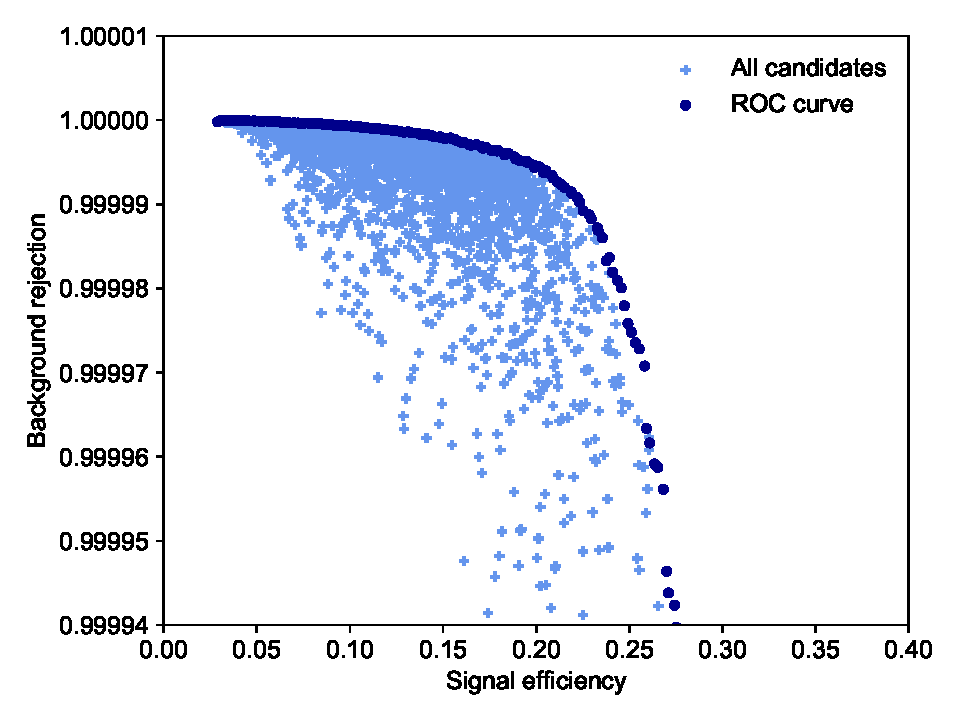
\includegraphics[width=1.0\textwidth]{N-1_cut_scan/roc_curve_thesis_plots}
		\caption{\label{fig:roc_curve}}
	\end{subfigure}\hfill
	\begin{subfigure}[b]{0.5\linewidth}
		\centering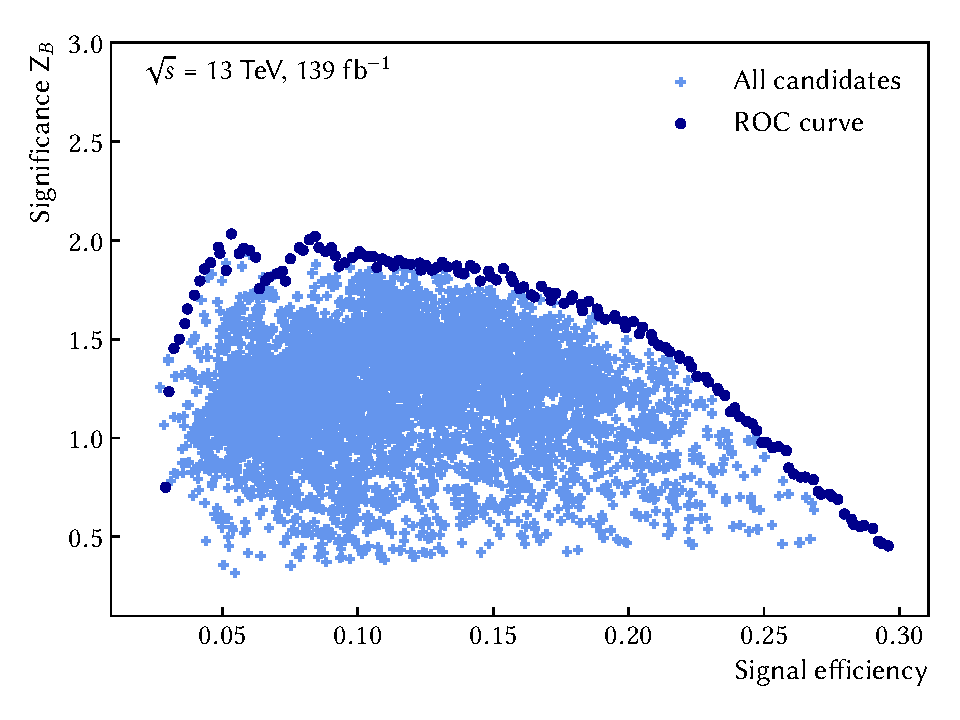
\includegraphics[width=1.0\textwidth]{N-1_cut_scan/z_vs_effs_thesis_plots}
		\caption{\label{fig:z_vs_eff}}
	\end{subfigure}\hfill

	\caption{Small $N$-dimensional cut scan using $10^4$ unique cut combinations, illustrating the approach of~\subref{fig:roc_curve} generating a \gls{roc} curve from the scanned cut combinations in order to \subref{fig:z_vs_eff} reduce the number of candidates used in computationally expensive significance calculations. In \subref{fig:z_vs_eff}, the significance $Z_\mathrm{B}$ includes the \gls{mc} statistical uncertainty on the expected background rate.} 
	\label{fig:ahoi_examples}
\end{figure}

\subsection{N-1 plots}\label{sec:n-1-scan}

Instead of performing a brute-force scan of a large set of cut combinations, a more manual approach, using repeated one-dimensional scans can be employed. In so-called $N-1$ plots, the variable distributions of the background components as well as exemplary signal processes are plotted together with the significance achieved by applying a cut on each value on the \textit{x}-axis of the plotted distribution. All other selection cuts except the one on the plotted variable are applied. This allows to investigate the impact that a cut on a single observable has on the overall significance value. By repeating this process for each variable considered, it is possible to iteratively approach a cut combination yielding results comparable to a brute-force cut scan. Especially when considering a sizeable set of variables, this manual approach quickly becomes very cumbersome and runs into the risk of missing optimal cut combinations an $N$-dimensional cut scan would have found.

For this reason, $N-1$ plots are used in the following to verify and fine-tune the results from $N$-dimensional cut scans.
 
\subsection{Fit scans}\label{sec:fit-scan}

The last of the optimisation methods used in the following relies on simplified fit setups in order to compute the expected exclusion limits for various signal region candidates obtained using the previous methods. The simplified fit setups estimate the background contribution purely from \gls{mc} and considers a systematic uncertainty on the background estimate of 30\%, correlated over all signal region bins. Statistical uncertainties on the background estimation from the limited \gls{mc} statistics are included for each bin. Similar to the previous methods, many different configurations can be tested, aiming to maximise the size of the expected exclusion contour.

Although being a very simple fit configuration, the statistical inference can take a significant amount of computation time. In order to keep the number of configurations to be tested at a manageable level, the signal region candidates obtained from the previous methods are only varied to a limited degree, assuming that they were already close to optimal in terms of expected exclusion area.

\section{Optimisation procedure}

\begin{table}
	\centering
	\small
	\setlength\heavyrulewidth{0.2ex}
	\caption[Cut ranges used in the $N$-dimensional cut scan]{List of observables and cut ranges used in the $N$-dimensional cut scan. All cut ranges, except for $N_\mathrm{jet}$ and $N_{b-\mathrm{jet}}$, are allowed not to be applied at all.}
	\begin{tabular} {l c l}
		\toprule
		Observable &  & Cut values \\ 
		\midrule
		$\etmiss$ [GeV]& $>$ & $\in \{200,220,240,260,280,300,320,340\}$ \\
		$\etmiss$ significance & $>$ & $\in \{5,10,15\}$ \\
		$\mt$ [GeV]& $>$ & $\in \{100, 120, 140,160,180,200,220,240,260,280, 300\}$ \\
		$\mct$ [GeV]& $>$ & $\in \{100, 120, 140,160,180,200,220,240,260,280, 300\}$ \\
		$m_\mathrm{bb}$ lower [GeV]& $>$ & $\in \{85,90,95,100,105,110,115\}$ \\
		$m_\mathrm{bb}$ upper [GeV]& $<$ & $\in \{130,135,140,145,150\}$ \\
		$p_\textrm{T}^\ell$ $[\SI{}{\GeV}]$& $>$ & $\in \{20, 40, 60, 80\}$ \\
		$p_\textrm{T}^\mathrm{jet1}$ [GeV]& $>$ & $\in \{50, 100, 150\}$ \\
		$p_\textrm{T}^\mathrm{jet2}$ [GeV]& $>$ & $\in \{50, 75, 100\}$ \\	
		$\Delta R_\mathrm{jj}$ & $<$ & $\in \{0.8,1.0,1.2,2.0\}$ \\
		$\Delta R_\mathrm{bb}$ & $<$ & $\in \{0.8,1.0,1.2,2.0\}$ \\
		$N_\mathrm{jet}$ & $\leq$ & $\in \{2,3,4\}$ \\			
		$\Delta\phi (\vetmiss,\vptlep )$ [rad]& $>$ & $\in \{0.5,1.0,2.0,2.5\}$ \\
		\bottomrule					
	\end{tabular}
	\label{tab:cut_scan}   
\end{table}

The optimisation of the \glspl{sr} uses experience from past analyses investigating the same signal model in the same final state~\cite{SUSY-2013-23,SUSY-2017-01}, all the while exploring new observables and \gls{sr} configurations optimised for the full Run~2 dataset. 

\subsection{Benchmark signal points}

A total of six so-called \textit{benchmark} signal points representative for the entire signal grid are chosen for the first step of the optimisation procedure involving $N$-dimensional cut scans and $N-1$ plots. Apart from the variables introduced in~\cref{sec:variables}, a set of additional, potentially discriminative observables are considered in the $N$-dimensional cut\improvement{Need presel plots for these} scan\footnote{These variables will turn out not to be used for the final signal regions and are only introduced here for completeness of the optimisation procedure description.}:
\begin{itemize}
	\item Transverse momenta of the two leading jets as well as the lepton. Especially for signal models with high mass differences between the $\charg/\neutr$ and the $\lsp$, the transverse momenta of the lepton and the jets tend to be higher than in background processes.
	\item Object-based $\etmiss$ significance $S$~\cite{met_significance:2294922}, a quantity designed to offer good discrimination against fake $\etmiss$ caused by mismeasurements or the non-hermeticity of the detector. Events with a large share of fake $\etmiss$ accumulate at low values of $S$, while events with mostly real $\etmiss$ tend to have large values of $S$. \unsure{is this conf up-to-date?}
	\item The distance between the two leading jets $\Delta R_\mathrm{jj}$ as well as the two \textit{b}-jets $\Delta R_\mathrm{bb}$. As the two \textit{b}-jets originating from the Higgs decay in the signal scenario tend to be close together and the highest-$\pt$ jets in an event, both $\Delta R_\mathrm{jj}$ and $\Delta R_\mathrm{bb}$ tend to have small values for signal events. In background processes, the two leading (\textit{b}-)jets often do not originate from the same object and thus tend to be further apart.
	\item The azimuthal distance between the lepton $\pt$ and the missing transverse momentum, $\Delta \phi (\boldsymbol{p}_\mathrm{T}^\ell, \boldsymbol{p}_\mathrm{T}^\mathrm{miss})$. This observable exploits the fact that the lepton and the $\etmiss$ tend to have a more back-to-back configuration in signal events than in many background processes where the lepton and the neutrino (often responsible for most of the $\etmiss$ in an event) often originate from the same $W$ boson.
\end{itemize}

\begin{figure}
	\centering
	\begin{subfigure}[b]{0.5\linewidth}
		\centering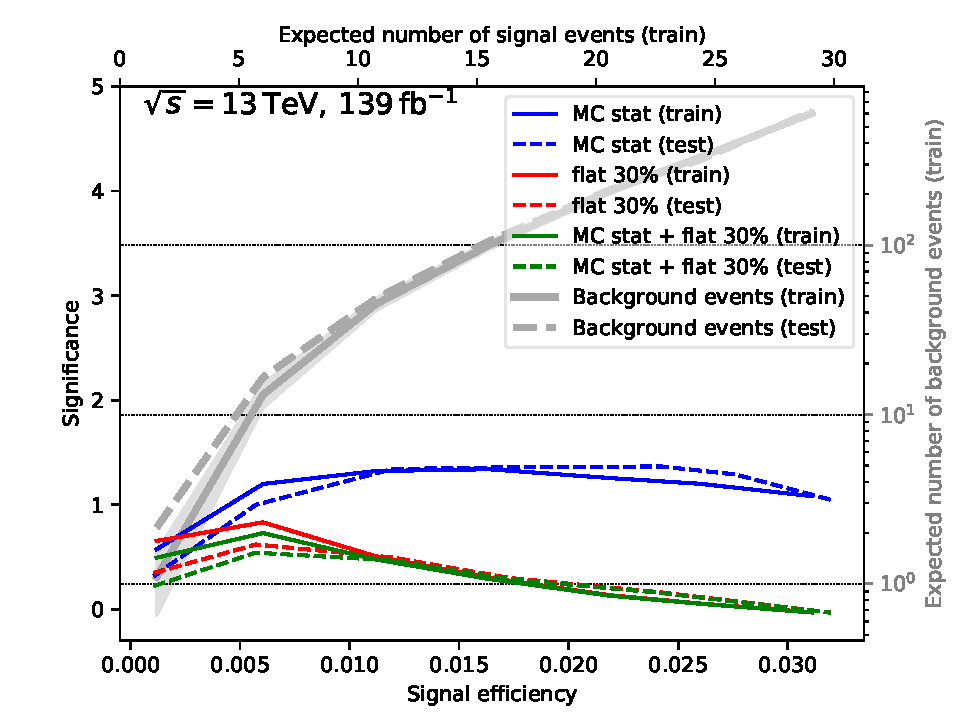
\includegraphics[width=1.0\textwidth]{N-1_cut_scan/z_vs_effs_300_150.pdf}
		\caption{}
	\end{subfigure}\hfill
	\begin{subfigure}[b]{0.5\linewidth}
		\centering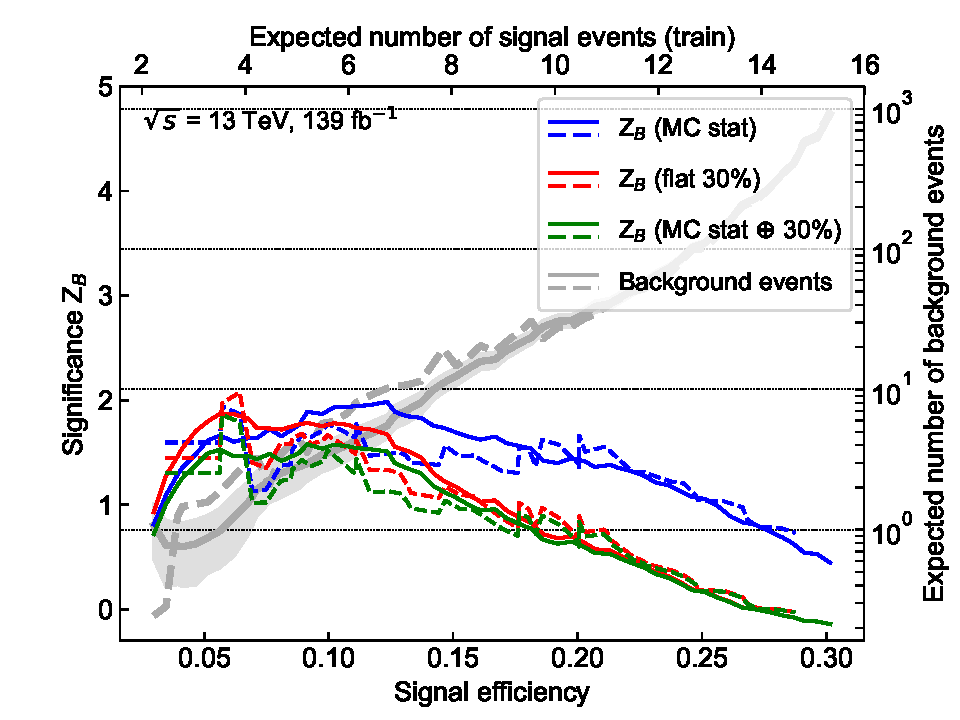
\includegraphics[width=1.0\textwidth]{N-1_cut_scan/z_vs_effs_800_250.pdf}
		\caption{}
	\end{subfigure}\hfill

	\caption[N-dimensional cut scan results]{Results of the $N$-dimensional cut scan for two exemplary benchmark points. The binomial discovery significance $Z_\mathrm{B}$ is plotted against the signal efficiency for varying uncertainty configurations. Additionally, the expected \gls{sm} background rates are shown, including statistical uncertainty for one of the two statistically independent samples (shaded area). The solid and dashed lines represent the two statistically independent subset that the \gls{mc} samples are split into.}
	\label{fig:results_z_vs_eff}
\end{figure}

In order to avoid selecting cut combination candidates with overtightened selection criteria compared to the available \gls{mc} statistics, constraints on the relative statistical uncertainty on the background and on the raw number of \gls{mc} events passing the cut combination candidates are applied. Cut combinations are only considered if they result in less than 50\% relative statistical uncertainty on the total background. In addition, all cut combinations need to result in at least 5 raw \gls{mc} events for each of the major backgrounds, $\ttbar$, single top and $\wjets$.

The discrete selection possibilities for each of the observables are shown in \cref{tab:cut_scan}. A preselection of one lepton and exactly two \textit{b}-jets (and thus at least two jets overall in the event) is always applied. Requirements on the different observables in~\cref{tab:cut_scan} are optional and do not need to be applied by the optimisation algorithm. The results of the brute-force $N$-dimensional cut scans for each benchmark signal point can be visualised by plotting the expected discovery significance $Z_\mathrm{B}$ against the signal efficiency. \Cref{fig:results_z_vs_eff} shows the cut scan results for two of the benchmark signal points, the corresponding plots for the remaining benchmark points can be found in~\cref{fig:results_z_vs_eff_rest}. In these figures, the binomial significance is calculated for different uncertainty configurations for each of the two statistically independent subsets. In addition, the expected background rate is shown for each of the two sample subsets. As such, these figures allow to pick a cut combination with high achieved significance while avoiding statistical fluctuations and overtightening. The cut combinations chosen for each benchmark point, after a round of $N-1$ plots, are shown in~\cref{tab:cut_scan_results}. The $N-1$ plots, shown in~\cref{fig:results_n1_800_0,fig:results_n1_800_150,fig:results_n1_800_250,fig:results_n1_600_300,fig:results_n1_400_200,fig:results_n1_300_150}, are used to validate and fine-tune the cut values obtained through the cut scan and allows to remove cuts on observables that do not contribute significantly to the achieved $Z_\mathrm{B}$ value. From the initially 12 considered observables, only six (excluding the \textit{b}-jet multiplicity technically not part of the scan) are part of the chosen cut combination candidates. The remaining observables turned out not to significantly improve the sensitivity.


\begin{table}
	\begin{center}
	\small
			\begin{tabular} {l c c c c c c c}
				\toprule
				Observable &  $(300,150)$ & $(400,200)$ & $(600,300)$  & $(800,250)$ & $(800,150)$ & $(800,0)$ \\
				\midrule
				$N_{b\mathrm{-jet}}$ &  2 & 2 & 2 & 2 & 2 & 2 \\
				$N_\mathrm{jet}$ & 2 & 2 & 2 -- 3 & 2 -- 3  & 2 -- 3 & 2 -- 3\\
				$\mbb$  $[\SI{}{\GeV}]$& $[105-135]$ & $[100-140]$ & $[100-140]$ & $[95-145]$ & $[95-145]$ & $[95-145]$ \\
				$\met$ $[\SI{}{\GeV}]$ & $>240$ & $>240$ & $>240$ & $>240$ & $>240$  & $>240$\\
				$m_\mathrm{CT}$ $[\SI{}{\GeV}]$ &  $>200$ & $>240$ & $>260$ & $>260$ & $>260$   & $>280$ \\
				$m_\mathrm{T}$ $[\SI{}{\GeV}]$ &  $>100$ & $>120$ & $>140$ & $>200$ & $>240$ & $>240$ \\
				$\mlb$ $[\SI{}{\GeV}]$ &  $-$ & $-$ & $>150$ & $>120$ & $>120$ & $>120$ \\
				\midrule
				$Z_\mathrm{B}$ $[\sigma]$ & \multicolumn{1}{c}{0.8} & \multicolumn{1}{c}{1.9} & \multicolumn{1}{c}{2.1} & \multicolumn{1}{c}{1.8} & \multicolumn{1}{c}{2.2} & \multicolumn{1}{c}{2.3} \\
				\bottomrule
			\end{tabular}
		\caption{Optimal cut combination for each benchmark signal point obtained with a brute force cut scan and a round of N-1 plots. The significance is computed for \onethirtynineifb with the binomial discovery significance $Z_\mathrm{B}$ and includes MC statistical uncertainty as well as a flat 30\% systematic uncertainty.}
		\label{tab:cut_scan_results}
	\end{center}
\end{table}




\subsection{Towards the final signal regions}

The optimal cut combinations obtained for the benchmark signal points, shown in~\cref{tab:cut_scan_results}, subsequently need to be consolidated into a finite set of \glspl{sr}. From~\cref{tab:cut_scan_results}, it can easily be seen that all benchmark points favour a baseline selection including exactly two \textit{b}-jets, possibly one additional light jet, a Higgs mass window requirement of roughly $\mbb\in [100,140]$~$\SI{}{\GeV}$, and $\etmiss > \SI{240}{\GeV}$. The requirements on $\mt$, $\mct$ and $\mlb$ are however not easily consolidated into a single signal region, as they vastly differ depending on the model space represented by each benchmark point.

From the normalised distributions in~\cref{fig:norm_obs}, it can already be seen that signal points from different kinematic regimes in the parameter space would in principle prefer different requirements on all three of these observables. Designing a single signal region that is optimised for the entire parameter space is thus not possible. Instead, a more generalised configuration is chosen, defining multiple signal region bins orthogonal to each other through their requirement on $\mt$ and the $\mct$, effectively creating a two-dimensional shape fit in these observables as the different \gls{sr} bins can be fit simultaneously. Such a shape-fit configuration allows to exploit the differences in shape between signal and background distributions, and is able to accommodate the varying shapes of signal points from different regions in the parameter space.

The optimal number of bins as well as values of the individual bin edges in both distributions depends on the available \gls{mc} statistics and is determined using the simplified fit scans introduced in~\cref{sec:fit-scan}. The \gls{mc} statistical uncertainty as well as a systematic uncertainty of 30\%, correlated over all bins, is considered in each scanned configuration. The number of bins are varied in each direction ($\mt$ and $\mct$) between two and five, each time with varying bin edge values. As configurations with more bins could benefit from the additional \gls{mc} statistics resulting from looser selection criteria on the remaining variables, the previously consolidated baseline selection is also allowed to vary to some extent. Configurations with multiple orthogonal \gls{sr} bins in the $\etmiss$ or $\mbb$ are also included in the scan. A subset of the investigated \gls{sr} candidates are shown in~\cref{fig:fit_scan_optimisation}, only showing the nominal expected exclusion limit at 95\% without uncertainty bands.

\begin{figure}
\floatbox[{\capbeside\thisfloatsetup{capbesideposition={right,center},capbesidewidth=0.35\textwidth}}]{figure}[\FBwidth]
{\caption{Expected exclusion contours obtained from a subset of the signal region candidates. The background estimation is taken directly from \gls{mc} and includes \gls{mc} statistical uncertainty as well as an uncorrelated shape uncertainty of 30\%. For the sake of visibility, only the nominal contours are shown (without uncertainty bands).}\label{fig:fit_scan_optimisation}}
{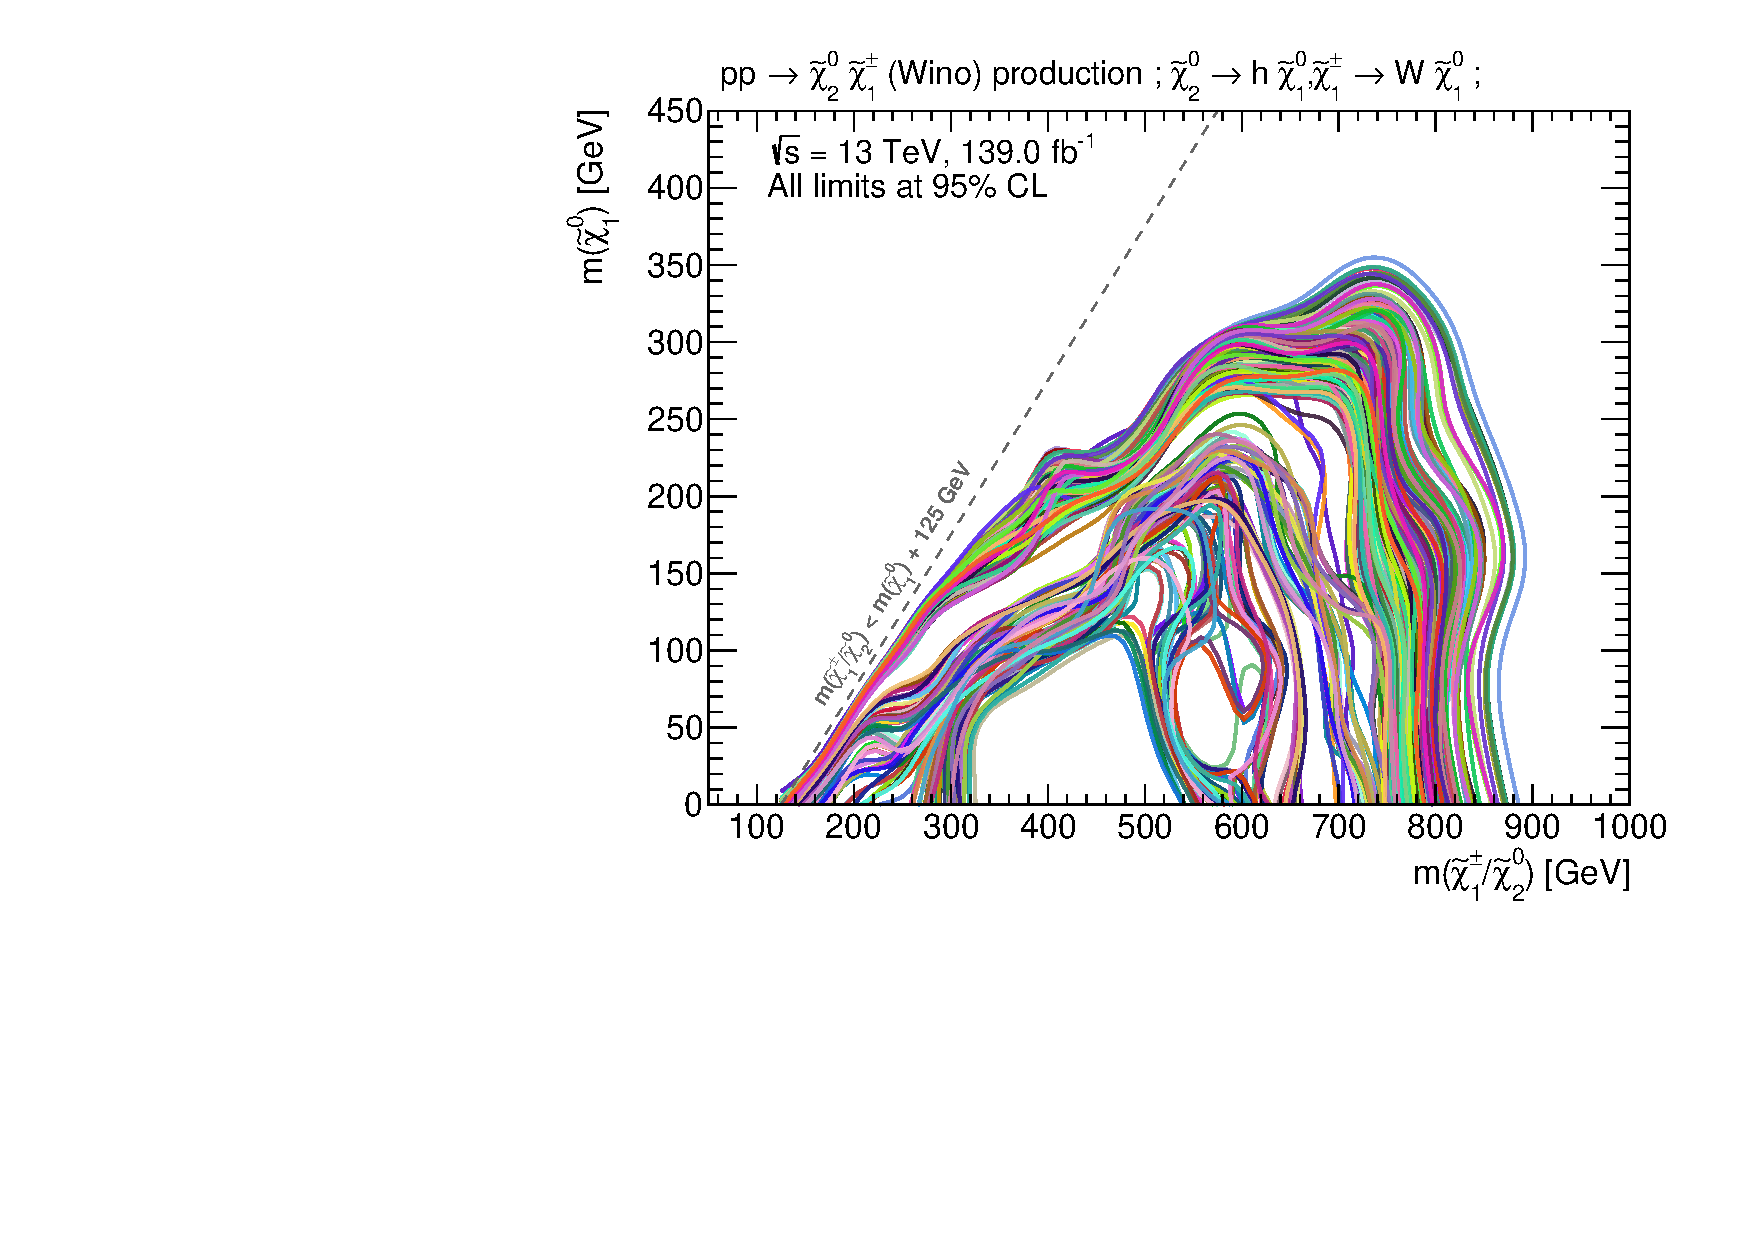
\includegraphics[width=0.6\textwidth]{HF/batch_compare}}
\end{figure}

As expected already from~\cref{tab:cut_scan_results}, the best performing configurations define multiple signal region bins in the $\mt$ and $\mct$ distributions, while keeping a constant baseline selection on the remaining observables. \Cref{fig:plot_binnings} shows a comparison of the expected exclusion contour for exemplary two-dimensional shape-fit configurations, using signal regions binned in ($\mt$, $\etmiss$), ($\mt$, $\mbb$) and ($\mt$, $\mct$). The setup using a two-dimensional shape-fit in $\mt$ and $\mct$ clearly maximises the expected excluded area. In addition, this configuration also leads to optimal sensitivity within the expected limit, as can be seen in~\cref{fig:plot_binnings_cls}. Finally, applying a requirement on high values of $\mlb$ in the highest $\mt$ bins has been shown (see~\cref{fig:plot_mlb1_cls}) to significantly improve sensitivity to signal models with high mass differences. 

 \begin{figure}
	\centering
	\begin{subfigure}[b]{0.5\linewidth}
		\centering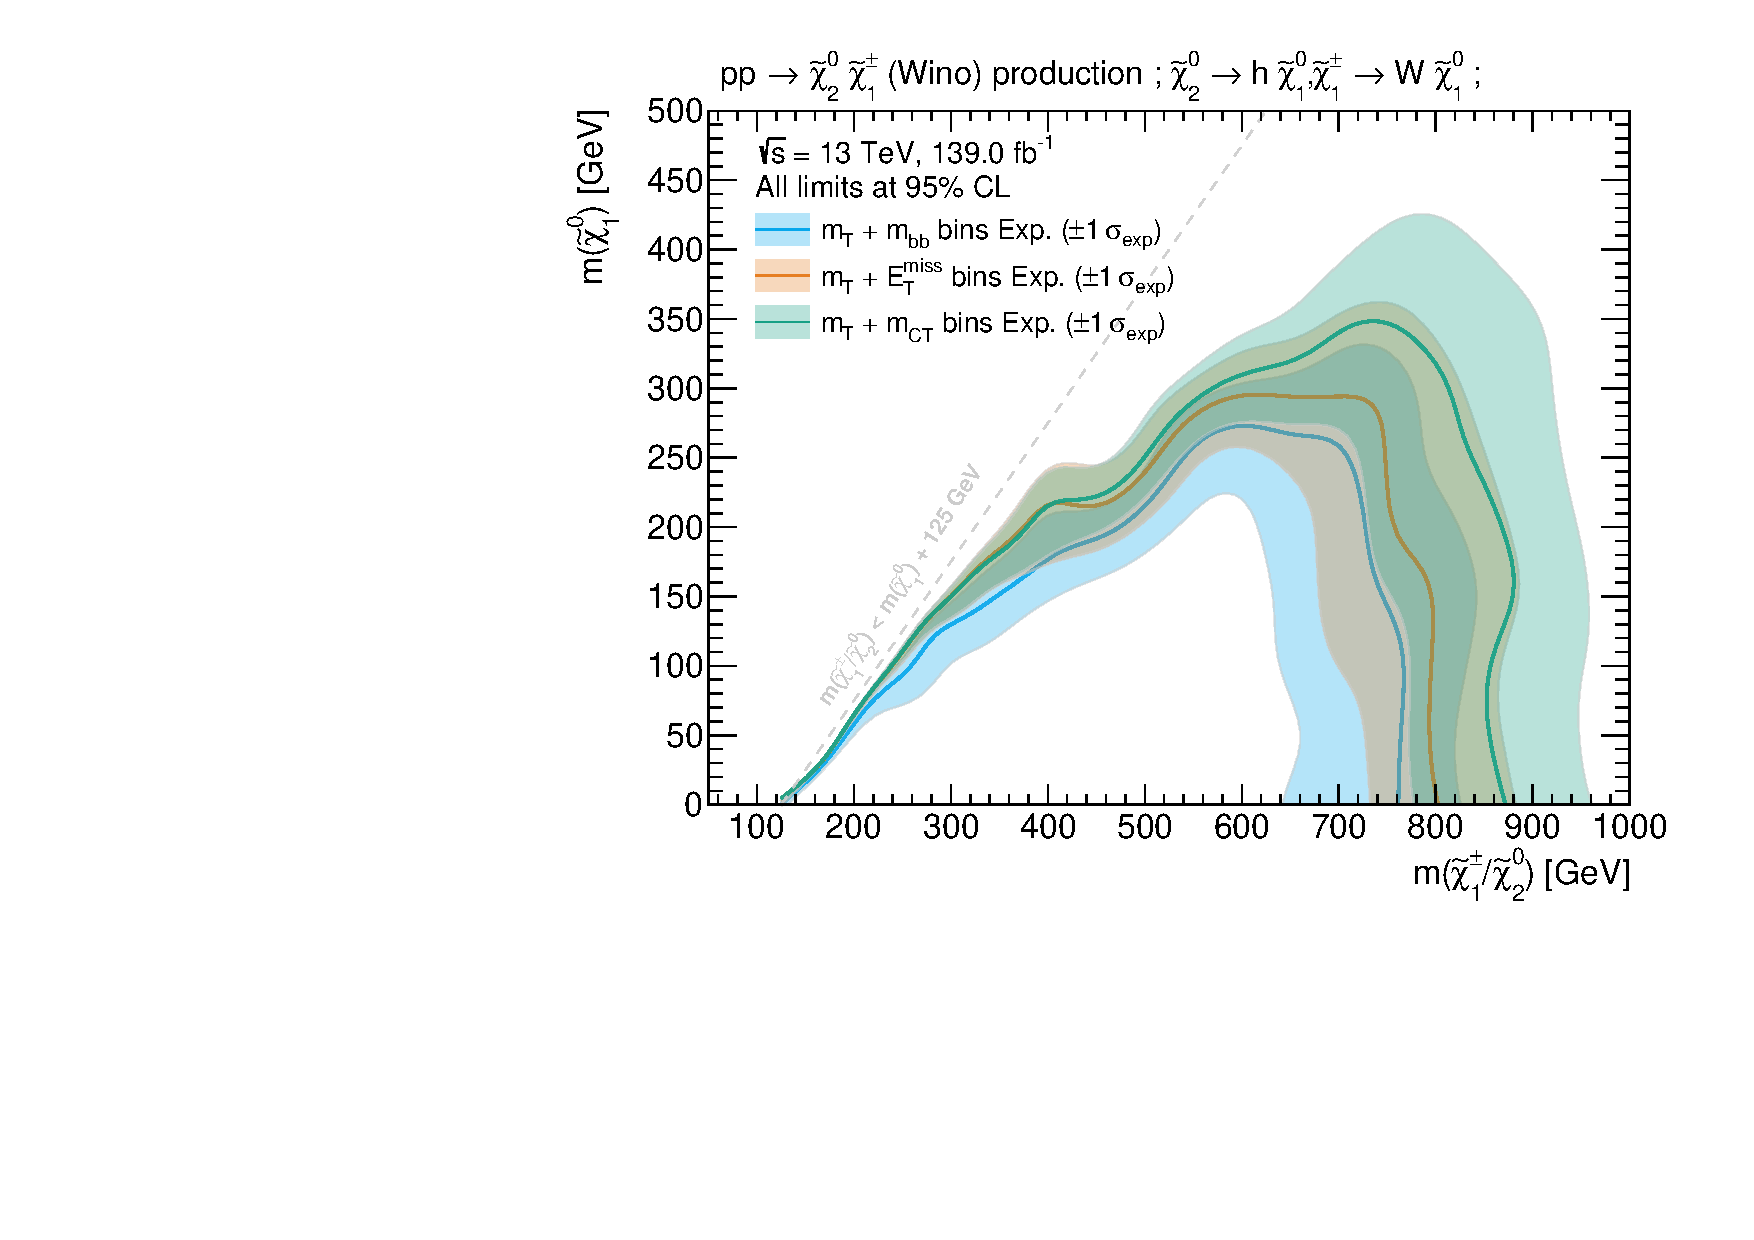
\includegraphics[width=1.0\textwidth]{HF/plot_binnings}
		\caption{\label{fig:plot_binnings}}
	\end{subfigure}\hfill
	\begin{subfigure}[b]{0.5\linewidth}
		\centering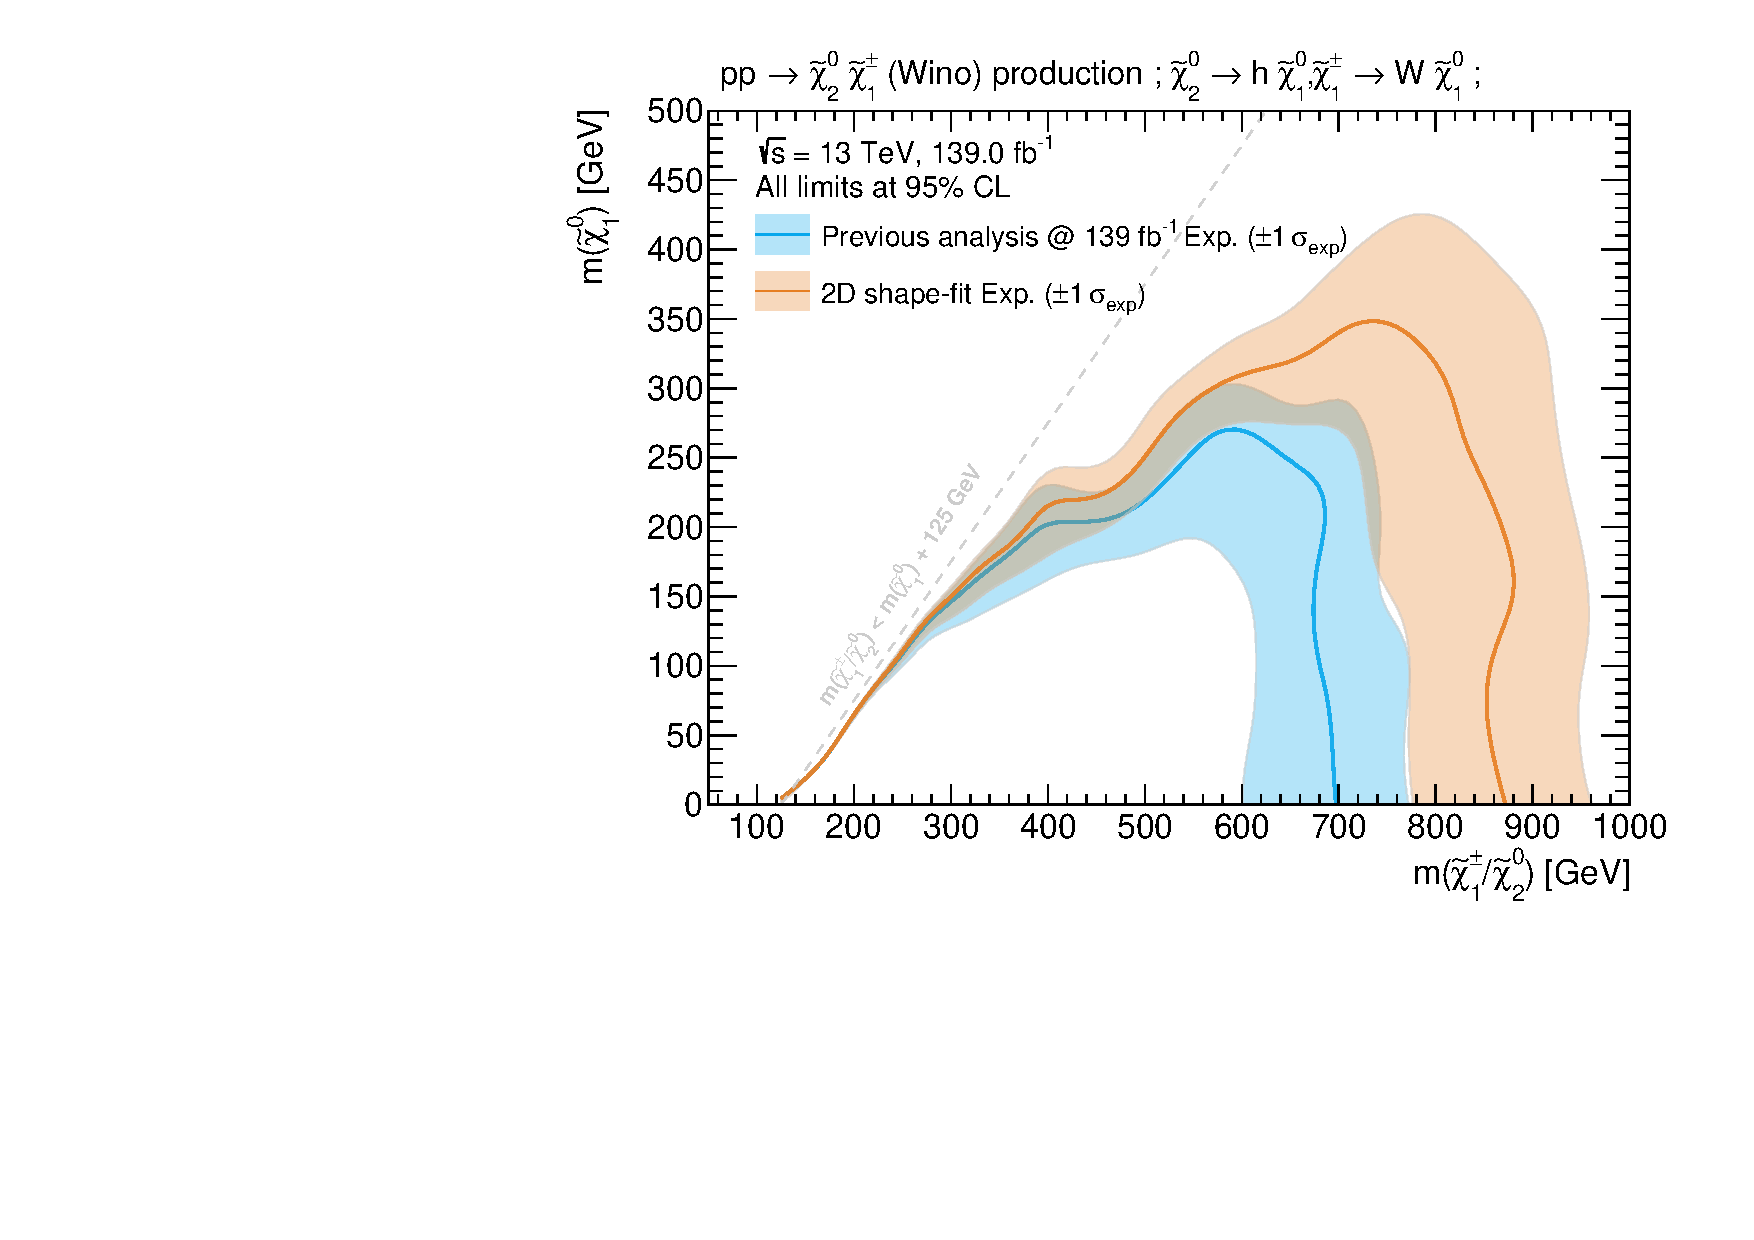
\includegraphics[width=1.0\textwidth]{HF/plot_2d_shapefit}
		\caption{}
	\end{subfigure}\hfill

	\caption{}
	\label{fig:results_HF_scans}
\end{figure}


\section{Signal region definitions}

An overview of the final signal region definitions is provided in~\cref{tab:SignalRegionDef}. Based on the previously discussed results, three signal regions bins in $\mt$ are defined, optimised for the low (SRLM), medium (SRMM), and high (SRHM) mass difference regimes. While SRLM targets the smallest values of $\mt$, SRMM and SRHM target progressively increasing values of $\mt$. All three signal regions are further divided into three $\mct$ bins each, resulting in a total of nine disjoint \gls{sr} bins. The signal region with the highest requirement on $\mt$ (SRHM) also requires $\mlb>\SI{120}{\GeV}$, for the reason explained previously. All three \glspl{sr} otherwise share a common set of requirements on the number of jets, $\etmiss$ and $\mbb$. As shape-fits are by construction highly model-dependent\footnote{The signal shapes need to be known in order to estimate the expected signal rates in multiple, disjoint signal region bins.}, these \glspl{sr} will be used for deriving model-dependent limits in the case where no significant excess compared to the expected \gls{sm} background rate is seen in data. For this reason, the shape-fit regions will be referred to as \textit{exclusion} regions in the following. A graphical representation of the nine exclusion signal region bins is shown in~\cref{fig:sr_strategy}.

For evaluating a potential excess in data compared to the expected background rate, a second set of signal regions is derived from the optimised shape-fit setup. For each of the three bins in the transverse mass (SRLM, SRMM, and SRHM), the three $\mct$ bins are summed up and the upper bound on $\mt$ is removed (if present). This results in three cut-and-count signal regions that make minimal model assumptions and can be interpreted in any signal model as long as the predicted signal rates are known. In case of no significant excess over the \gls{sm} expectation, these so-called \textit{discovery} \glspl{sr} can be used to derive model-independent limits. 

\begin{table}
	\begin{center}
		\begin{tabular} {l | c c c }
			\toprule
				&  \textbf{SRLM} & \textbf{SRMM} & \textbf{SRHM} \\
			\midrule
			$N_{\mathrm{lepton}}$ & \multicolumn{3}{c}{$=$ 1}\\
			$\ptl$ [\GeV] & \multicolumn{3}{c}{ $>7(6)$ for $e$($\mu$)} \\
			$N_\mathrm{jet}$ & \multicolumn{3}{c}{$=$ 2 or 3}\\
			$N_{b\textrm{-jet}}$ &\multicolumn{3}{c}{$=$ 2} \\
			$\met$ $[\SI{}{\GeV}]$ & \multicolumn{3}{c}{$>240$}\\
			$\mbb$  $[\SI{}{\GeV}]$ & \multicolumn{3}{c}{$\in [100,140]$}\\
			$m(\ell,b_1)$ $[\SI{}{\GeV}]$ & -- & -- & $>120$ \\
			\midrule
			%                        \mt $[\SI{}{\GeV}]\mathrm{(excl.)}$&   $\in [100,160]$ & $\in [160,240]$ & $\in [240,\infty]$ \\
			$\mt$ $[\SI{}{\GeV}]~\mathrm{(excl.)}$&   $\in [100,160]$ & $\in [160,240]$ & $>240$ \\
			
			
			$\mct$ $[\SI{}{\GeV}]~\mathrm{(excl.)}$ &\multicolumn{3}{c}{ $ \{ \in [180,230]$,\,$\in [230,280]$, $>280  \}$}\\
			%                        &\multicolumn{3}{c}{ $\in [180,230]$}\\
			%                        \mct $[\SI{}{\GeV}]\mathrm{(excl.)}$ & \multicolumn{3}{c}{ $\in [230,280]$} \\   
			%                         & \multicolumn{3}{c}{ $>280$}\\
			%                         & \multicolumn{3}{c}{ $\in [280,\infty]$}\\
			
			\midrule
			$\mt$ $[\SI{}{\GeV}]~\mathrm{(disc.)}$&   $>100$ & $>160$ & $>240$ \\
			$\mct$ $[\SI{}{\GeV}]~\mathrm{(disc.)}$ & \multicolumn{3}{c}{ $>180$}\\
			\bottomrule
		\end{tabular}
		\caption{Overview of the selection criteria for the signal regions. \textit{Exclusion} \glspl{sr} are defined for model-dependent limits, and \textit{discovery} \glspl{sr} are defined for model-independent limits. Each of the three exclusion \glspl{sr} is binned in three $\mct$ regions for a total of nine exclusion bins.} 
		\label{tab:SignalRegionDef}
	\end{center}
\end{table}

\begin{figure}
\floatbox[{\capbeside\thisfloatsetup{capbesideposition={right,center},capbesidewidth=0.35\textwidth}}]{figure}[\FBwidth]
{\caption{Configuration of the exclusion signal regions. Nine signal region bins are defined on $\mt$ and $\mct$ within the Higgs mass window, resulting in a two-dimensional shape-fit.}\label{fig:sr_strategy}}
{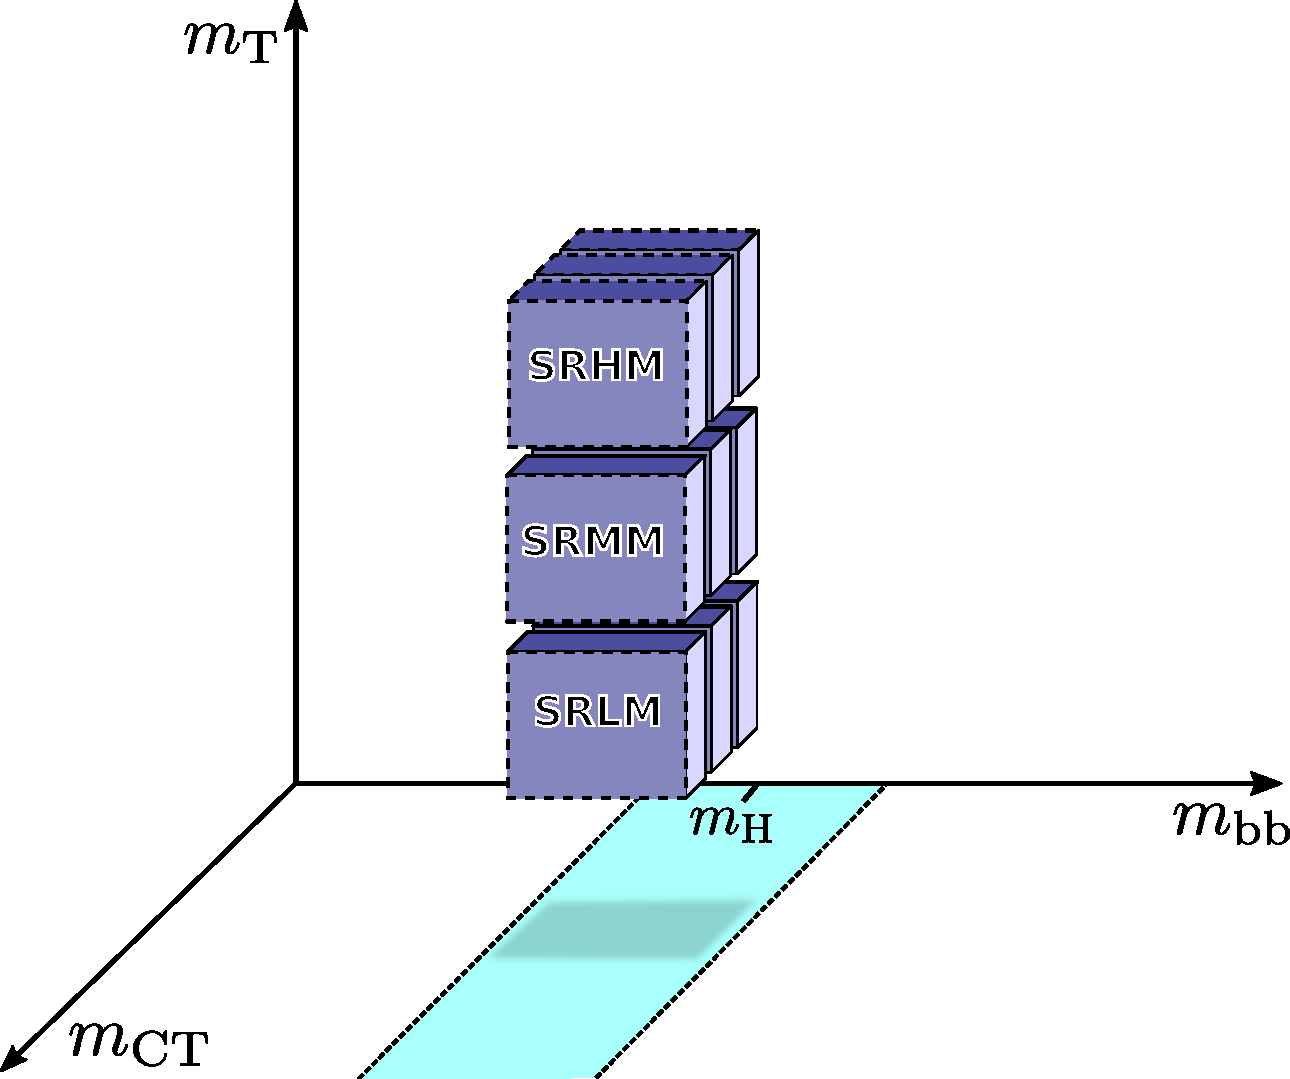
\includegraphics[width=0.6\textwidth]{strategy_2}}
\end{figure}


\begin{figure}
	\centering
	\begin{subfigure}[b]{0.4\linewidth}
		\centering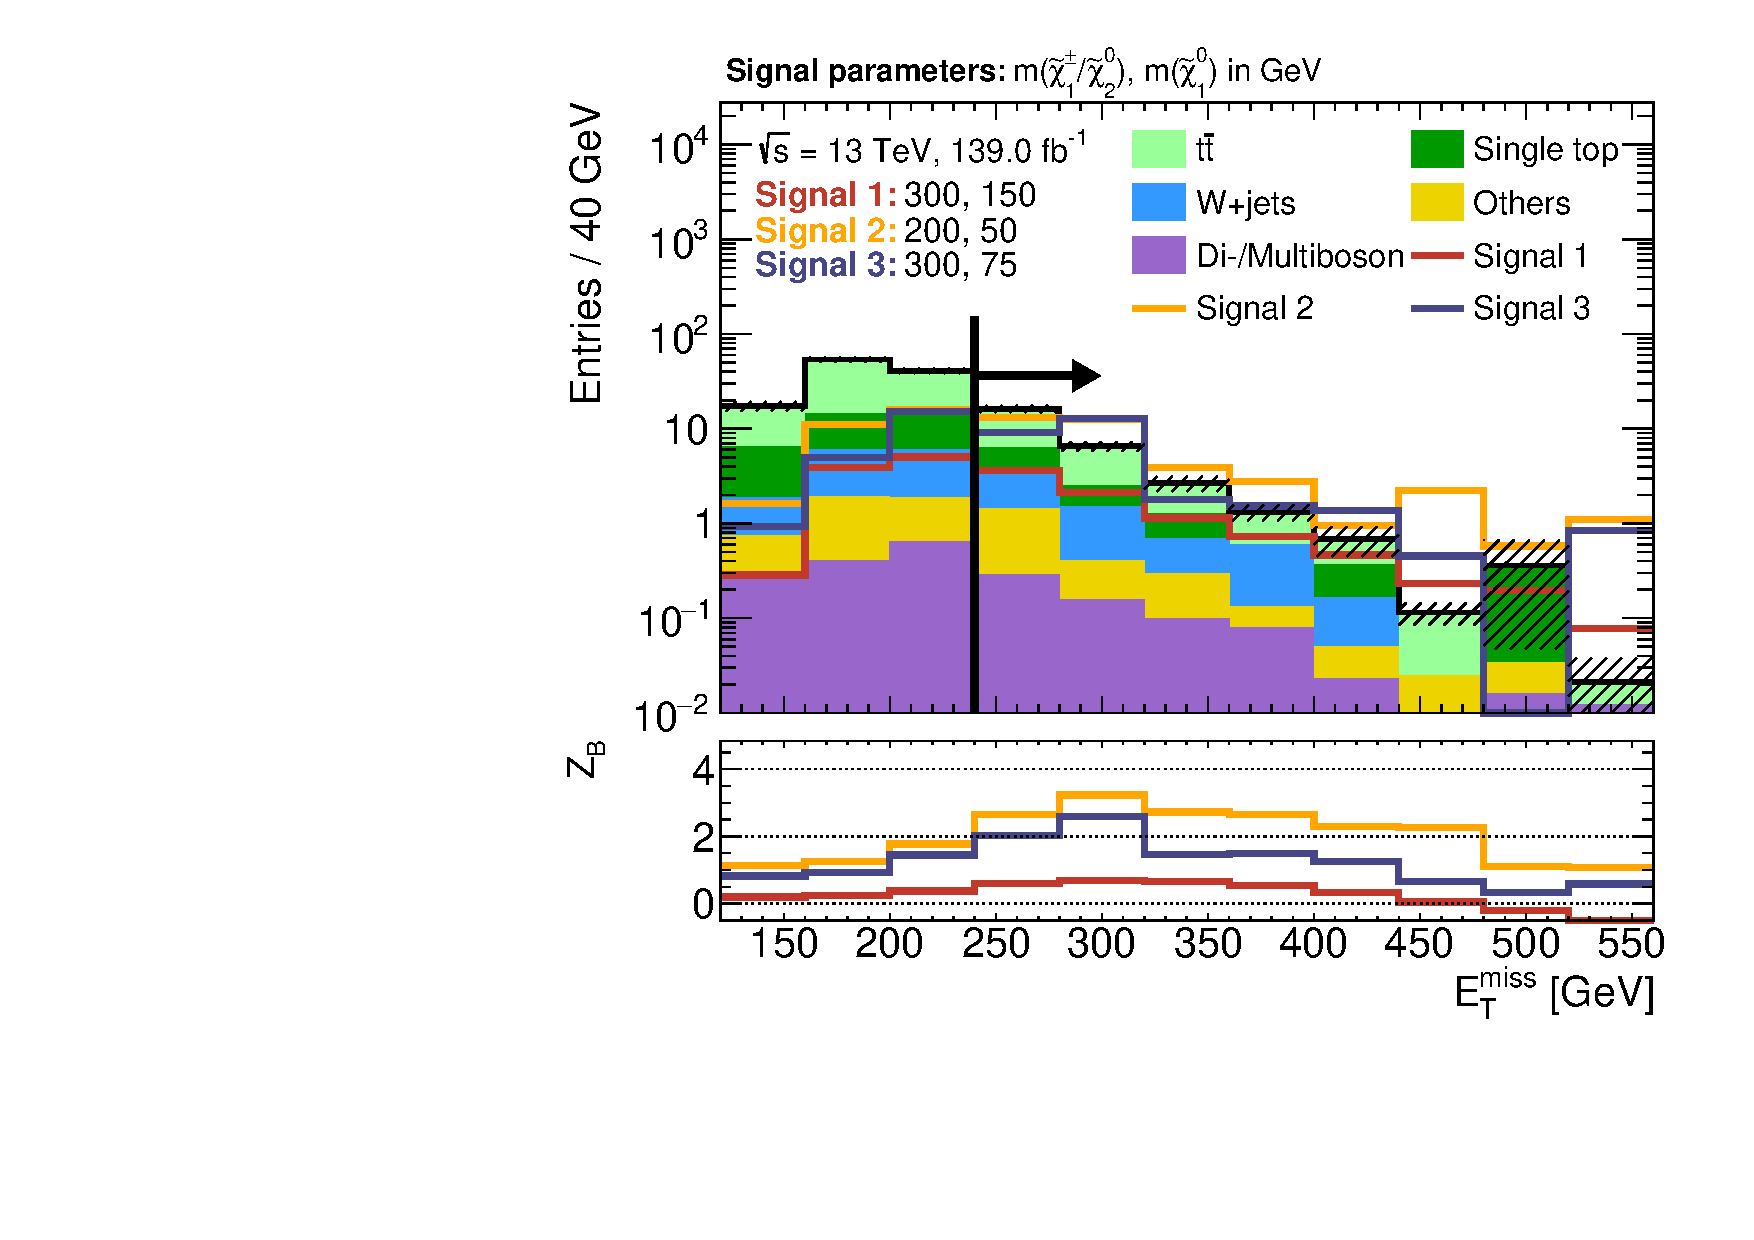
\includegraphics[width=\textwidth]{n1_SRLM_mct_bins/met.pdf}
		\caption{\label{fig:Wh_reopt_second_round_n1_srlm_met}}
	\end{subfigure}%
	\begin{subfigure}[b]{0.4\linewidth}
		\centering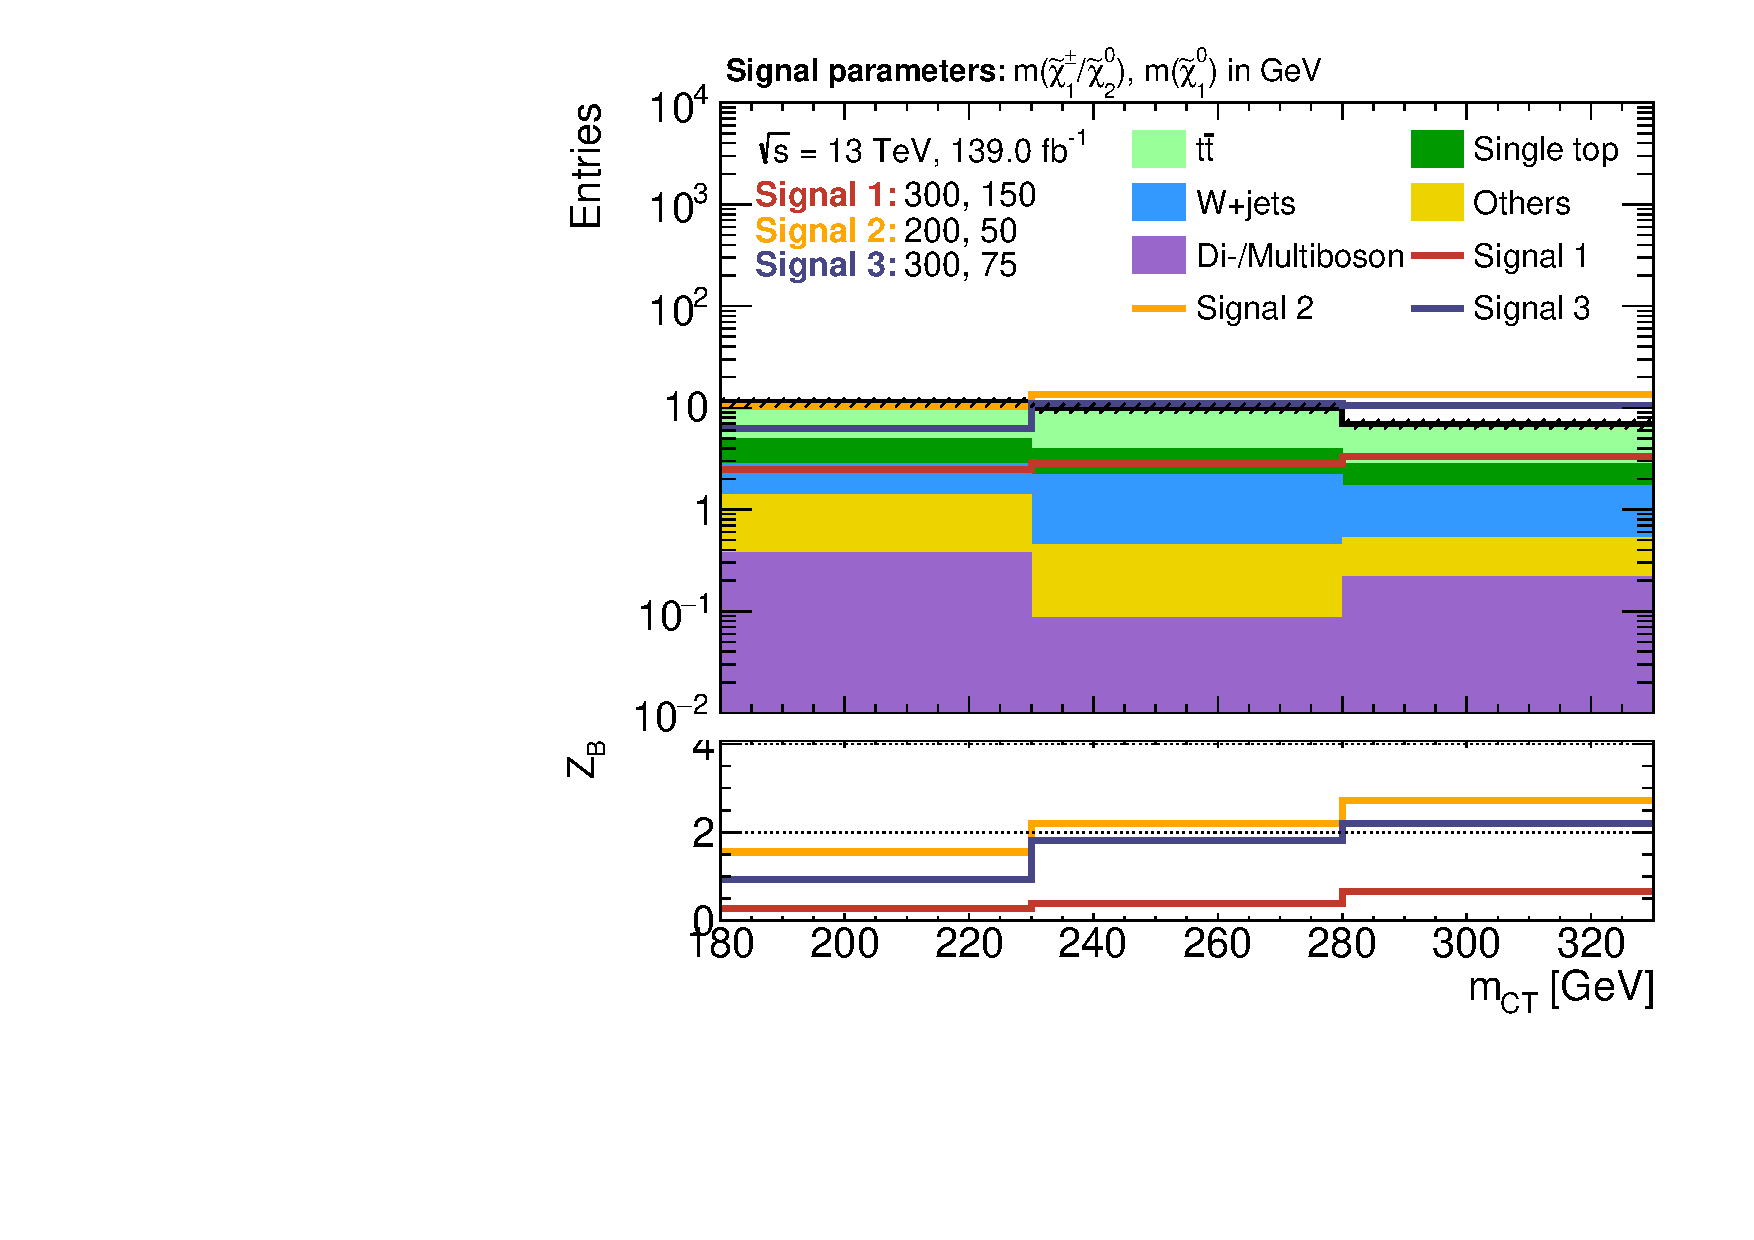
\includegraphics[width=\textwidth]{n1_SRLM_mct_bins/mct.pdf}
		\caption{\label{fig:Wh_reopt_second_round_n1_srlm_mct}}
	\end{subfigure}
	\begin{subfigure}[b]{0.4\linewidth}
		\centering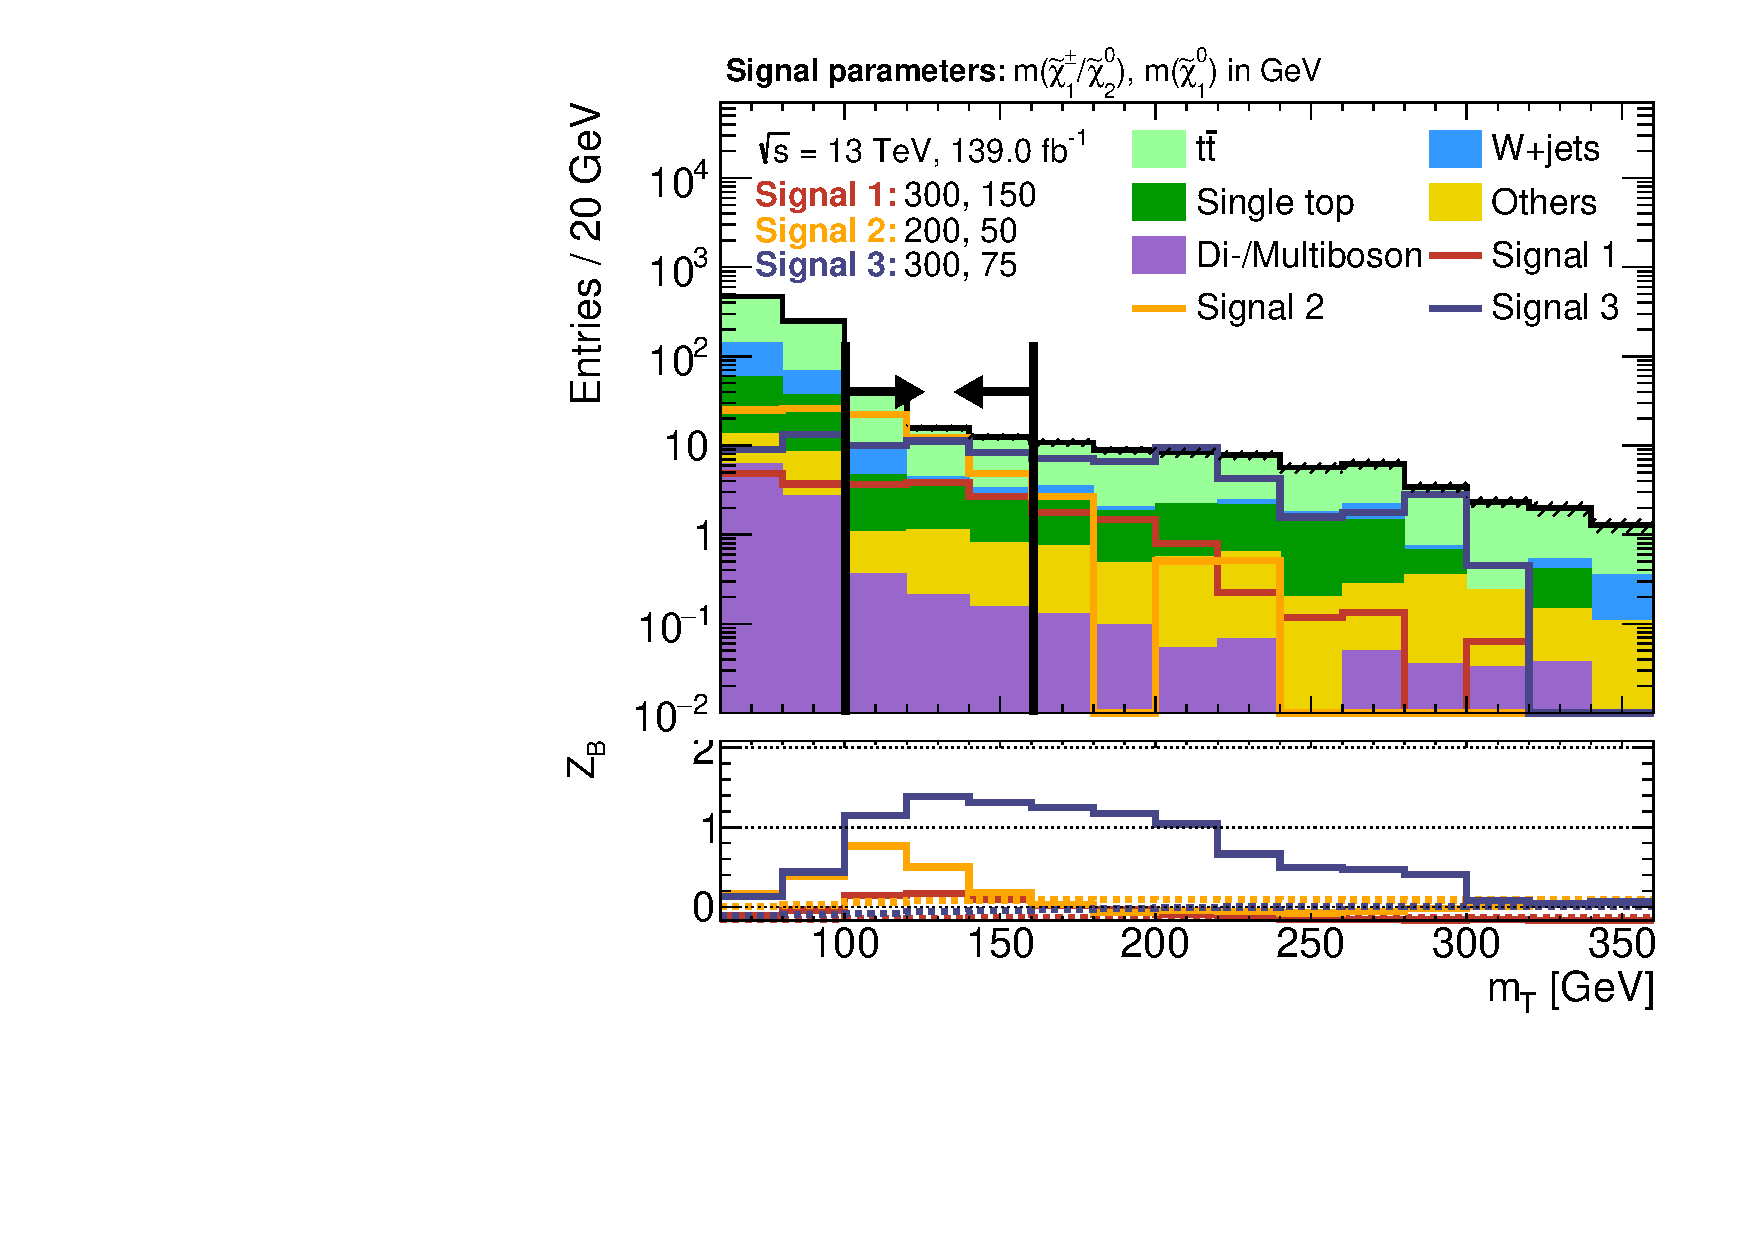
\includegraphics[width=\textwidth]{n1_SRLM_mct_bins/mt_both.pdf}
		\caption{\label{fig:Wh_reopt_second_round_n1_srlm_mt}}
	\end{subfigure}%
	\begin{subfigure}[b]{0.4\linewidth}
		\centering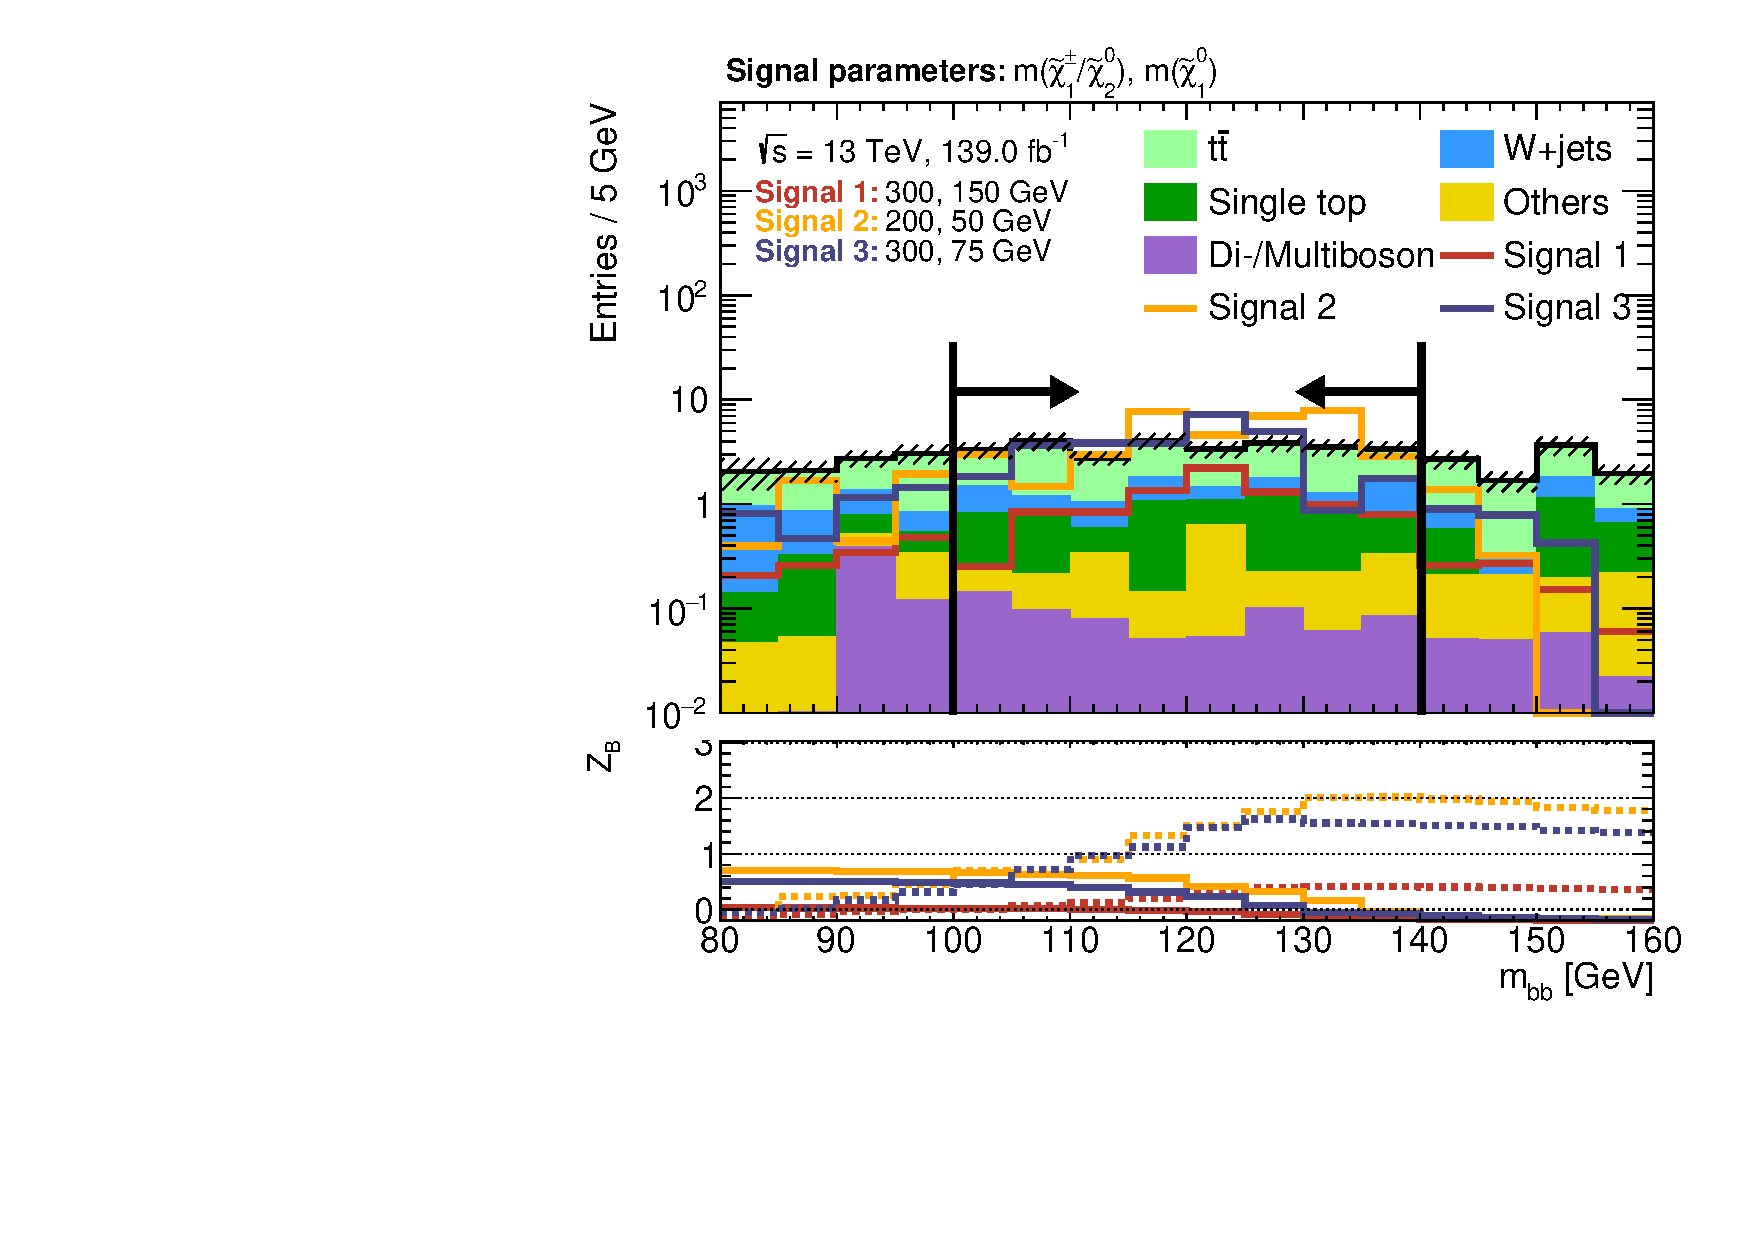
\includegraphics[width=\textwidth]{n1_SRLM_mct_bins/mbb_both.pdf}
		\caption{\label{fig:Wh_reopt_second_round_n1_srlm_mbb}}
	\end{subfigure}
%	\begin{subfigure}[b]{0.4\linewidth}
%		\centering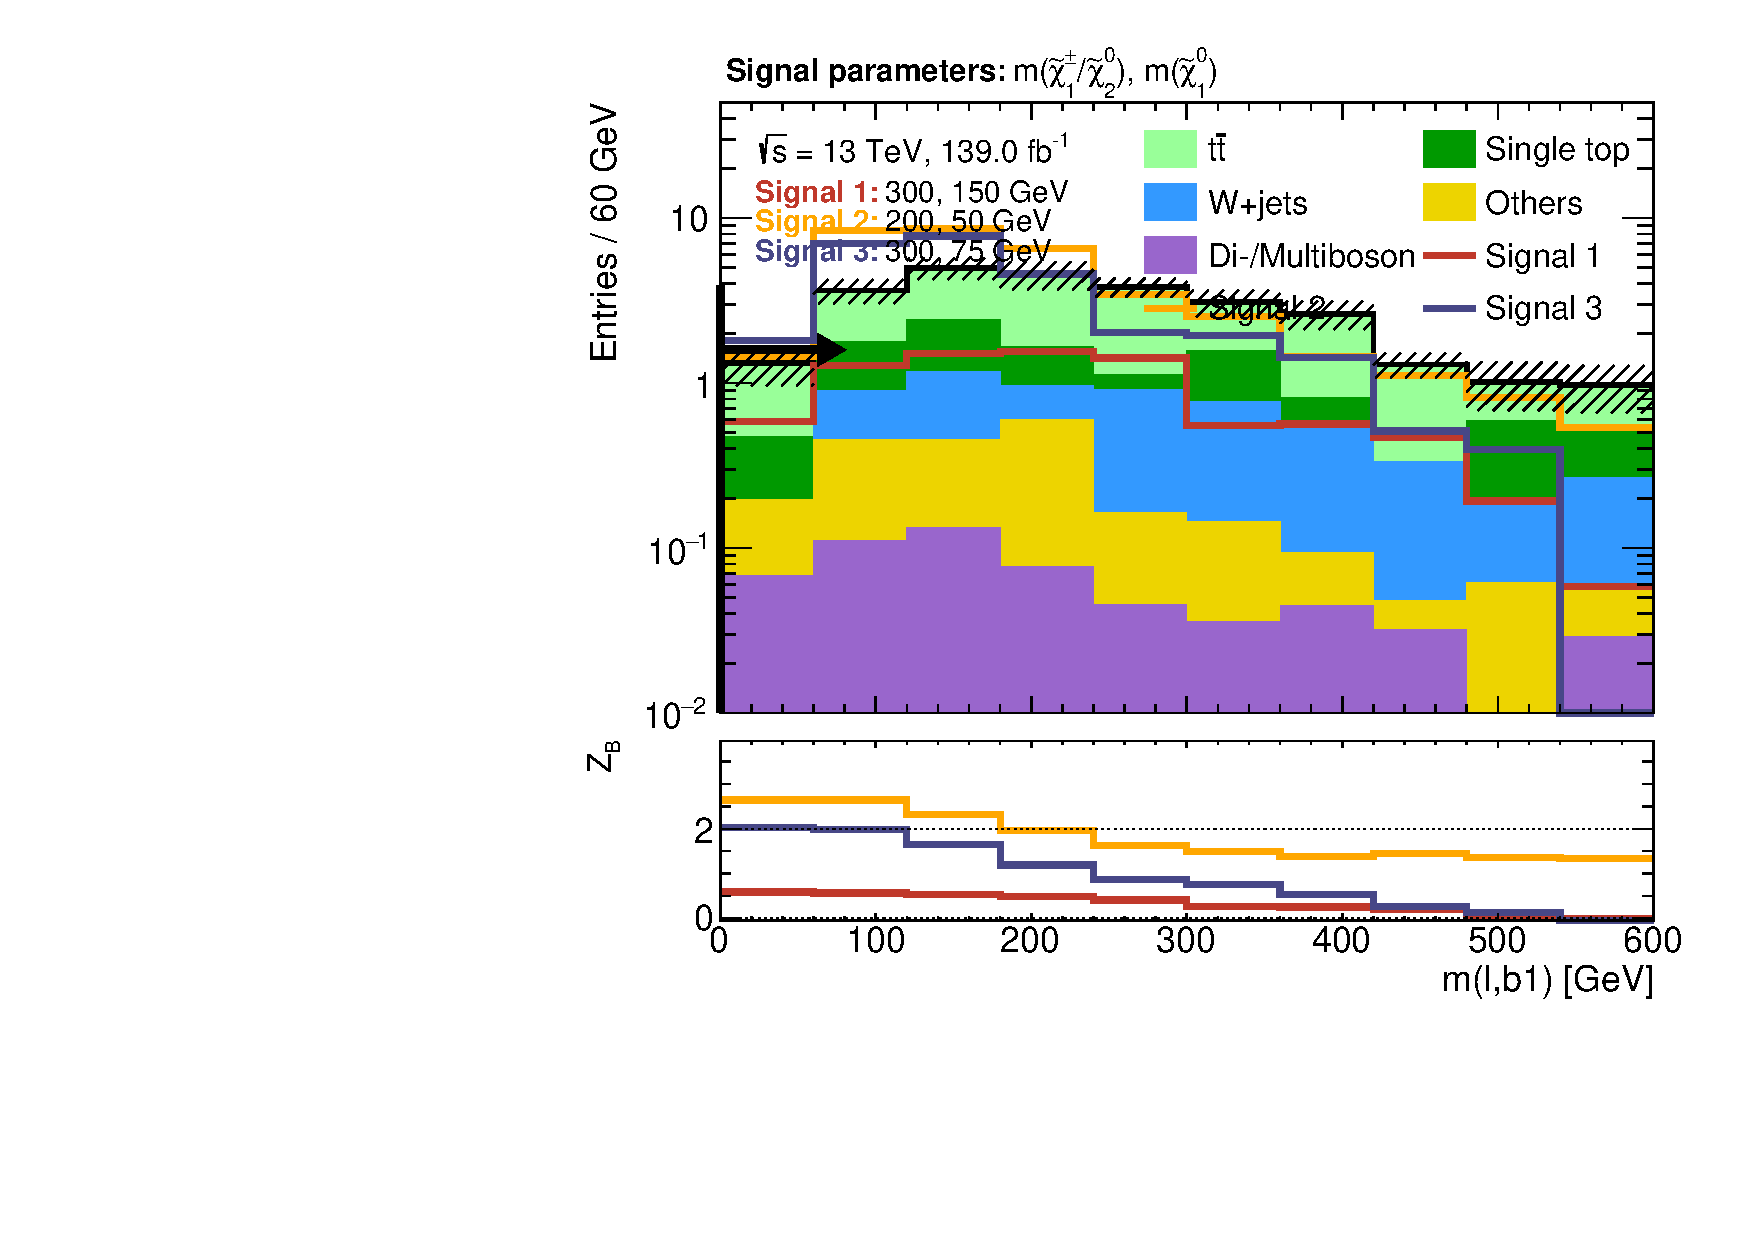
\includegraphics[width=\textwidth]{n1_SRLM_mct_bins/mlb1.pdf}
%		\caption{\label{fig:Wh_reopt_second_round_n1_srlm_mlb1}}
%	\end{subfigure}%
	\begin{subfigure}[b]{0.4\linewidth}
		\centering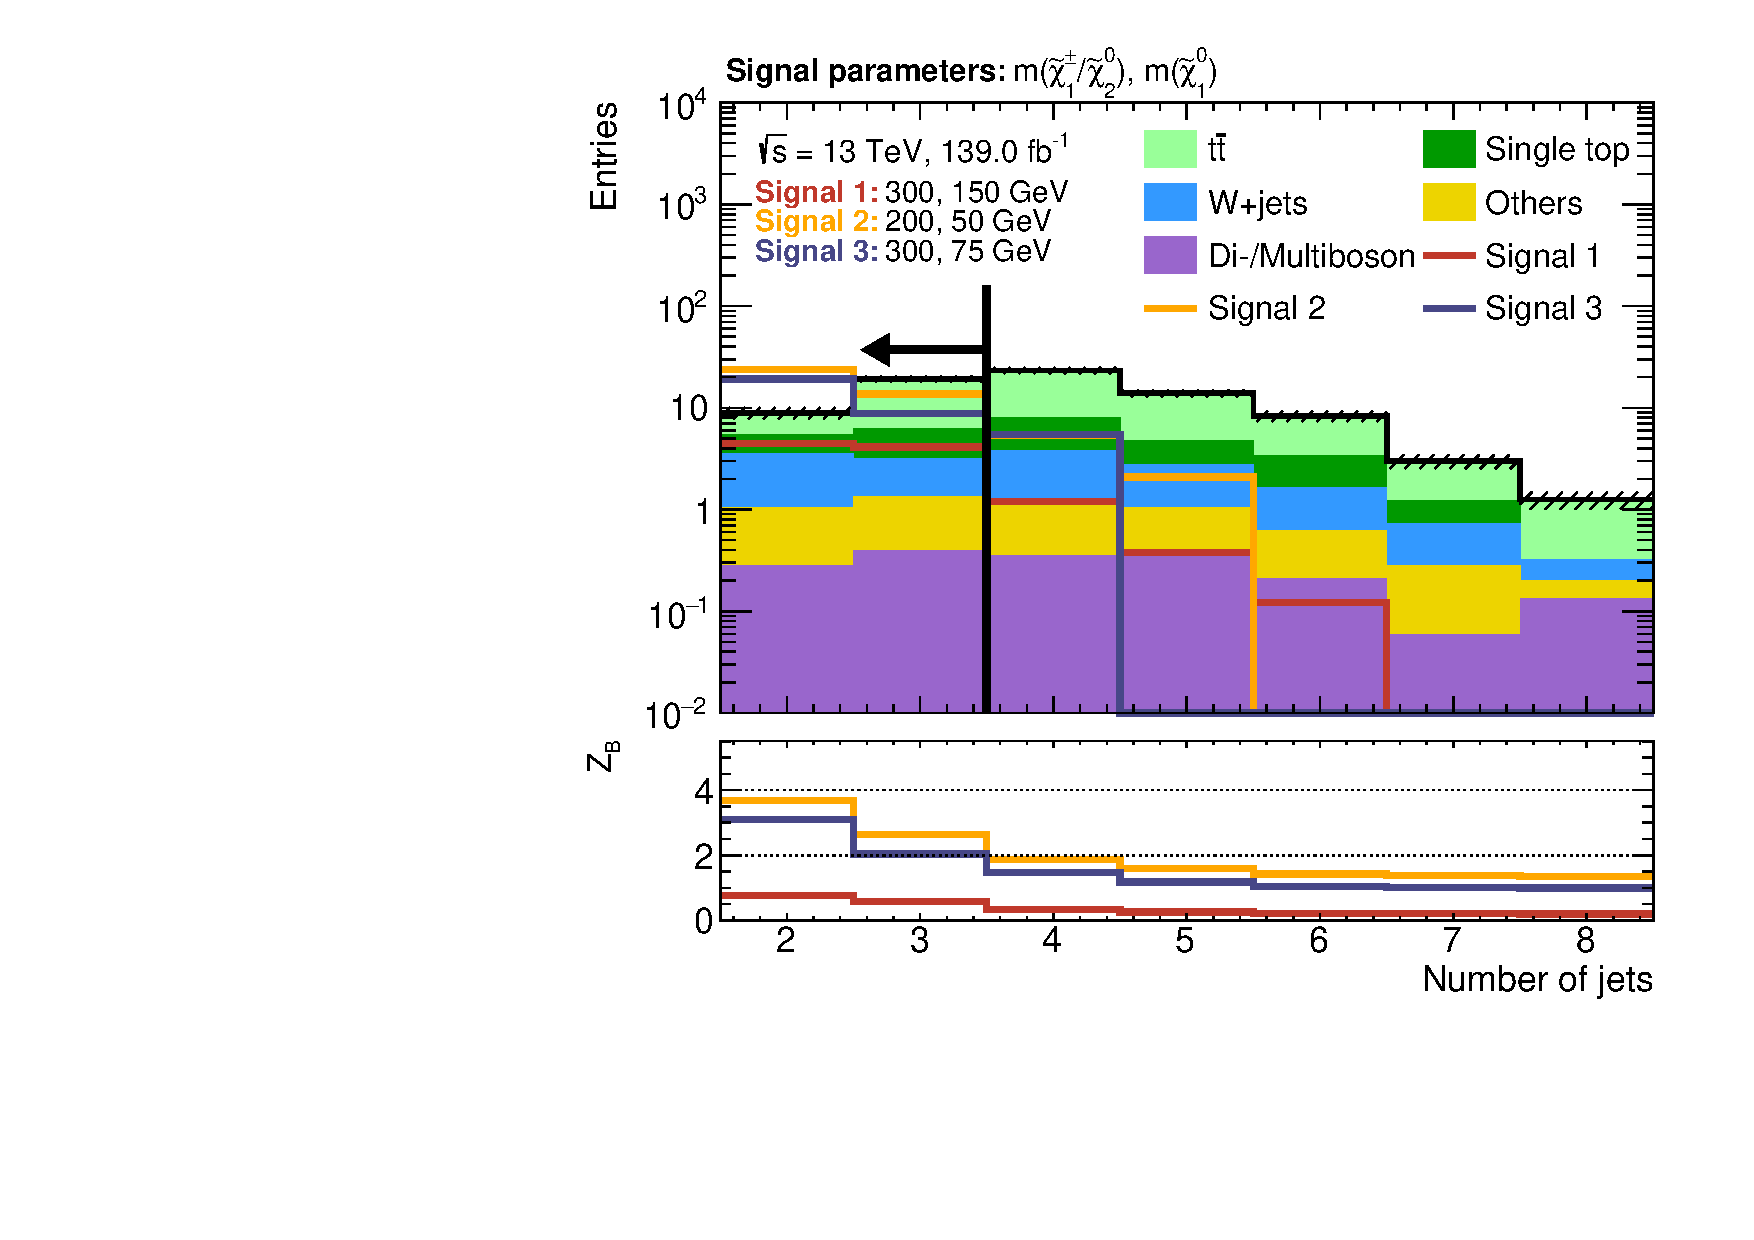
\includegraphics[width=\textwidth]{n1_SRLM_mct_bins/nJet30.pdf}
		\caption{\label{fig:Wh_reopt_second_round_n1_srlm_njet}}
	\end{subfigure}
	\caption{$N-1$ plots for SRLM, with exemplary signal points and all $\mct$ bins included. The dashed area represents \gls{mc} statistical uncertainty on the background. In all figures except \figname~\subref{fig:Wh_reopt_second_round_n1_srlm_mct}, the significance in the lower pad is obtained by summing up all the events in the direction of the cut arrow and includes 30\% uncertainty as well as MC statistical uncertainty. In \figname~\subref{fig:Wh_reopt_second_round_n1_srlm_mct} the significance is only computed on a bin-by-bin basis, \ie not summing up all events in the direction of the cut arrow.}
	\label{fig:Wh_reopt_second_round_n1_srlm}
\end{figure}

\begin{figure}
	\centering
	\begin{subfigure}[b]{0.4\linewidth}
		\centering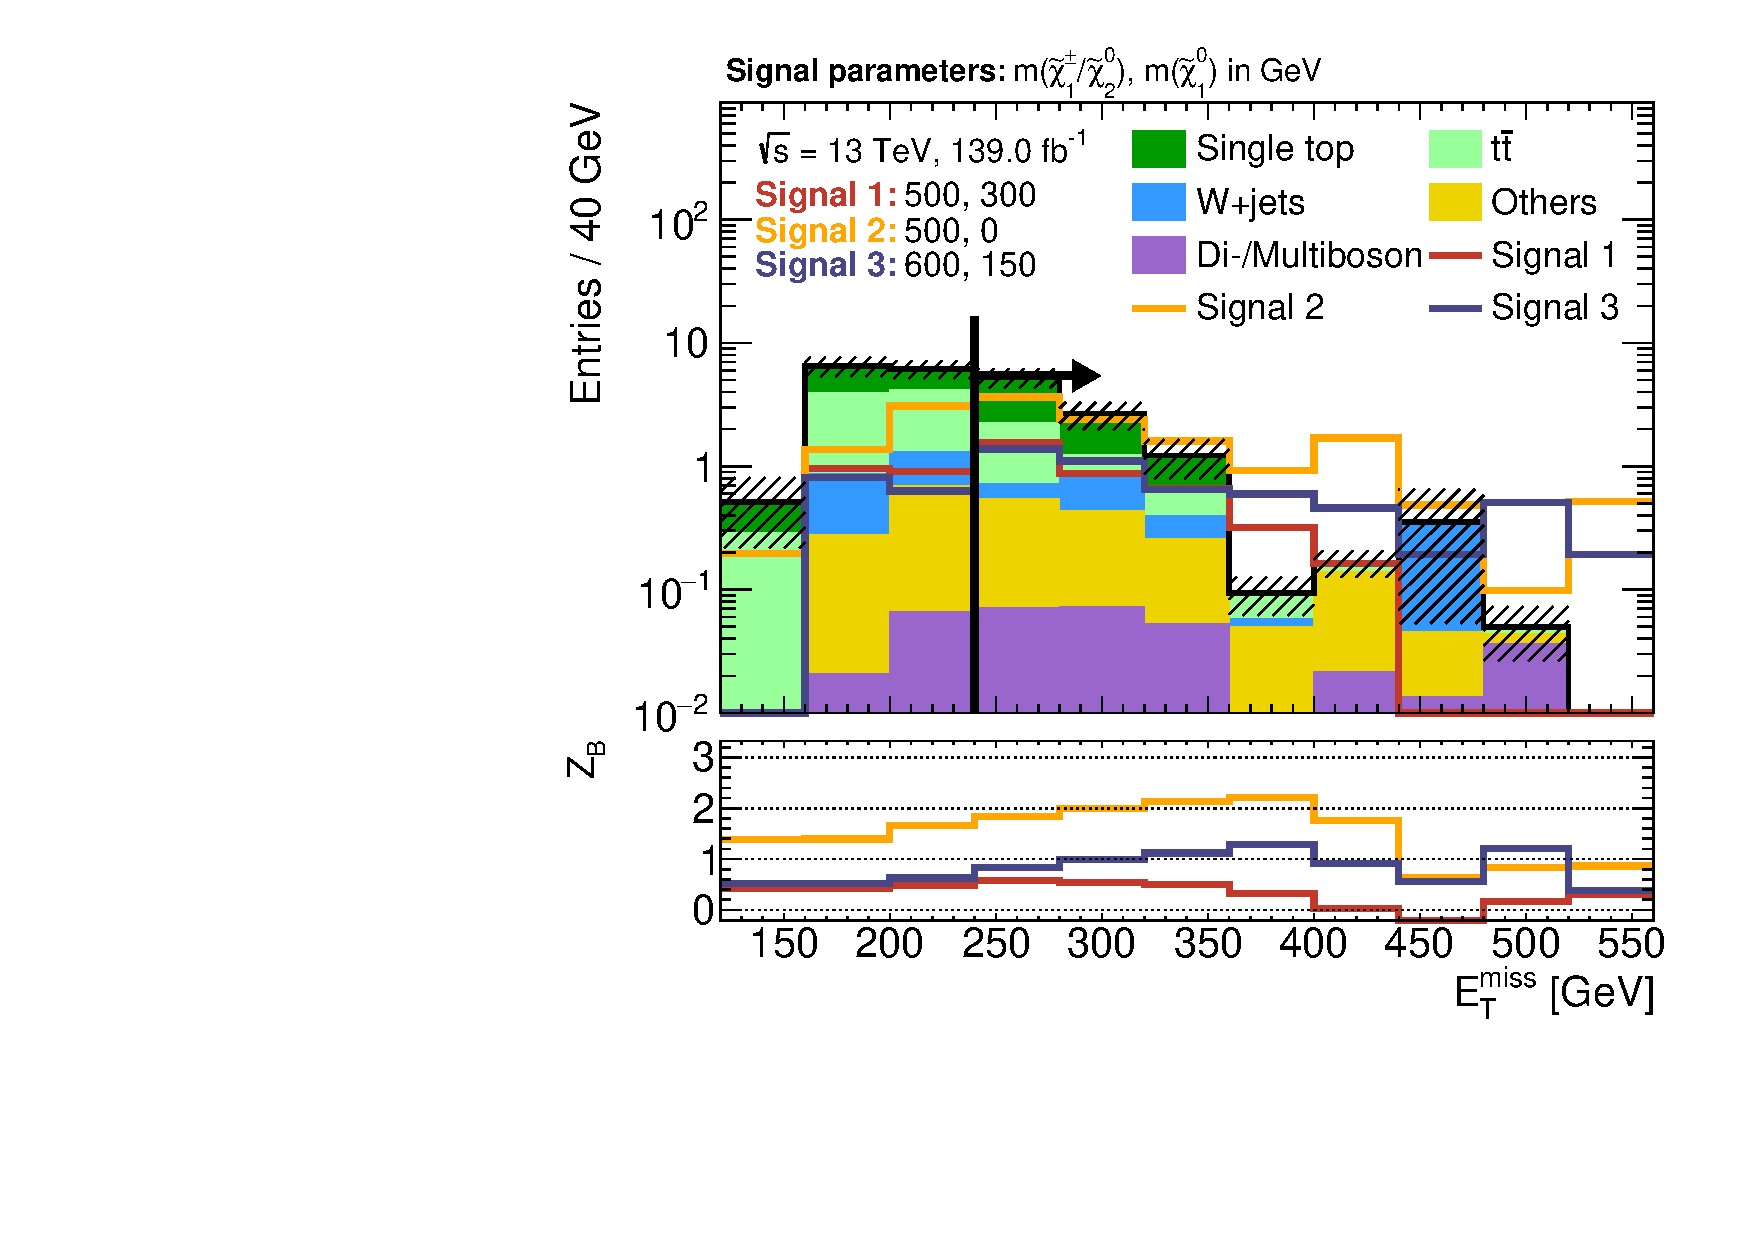
\includegraphics[width=\textwidth]{n1_SRMM_mct_bins/met.pdf}
		\caption{\label{fig:Wh_reopt_second_round_n1_srmm_met}}
	\end{subfigure}%
	\begin{subfigure}[b]{0.4\linewidth}
		\centering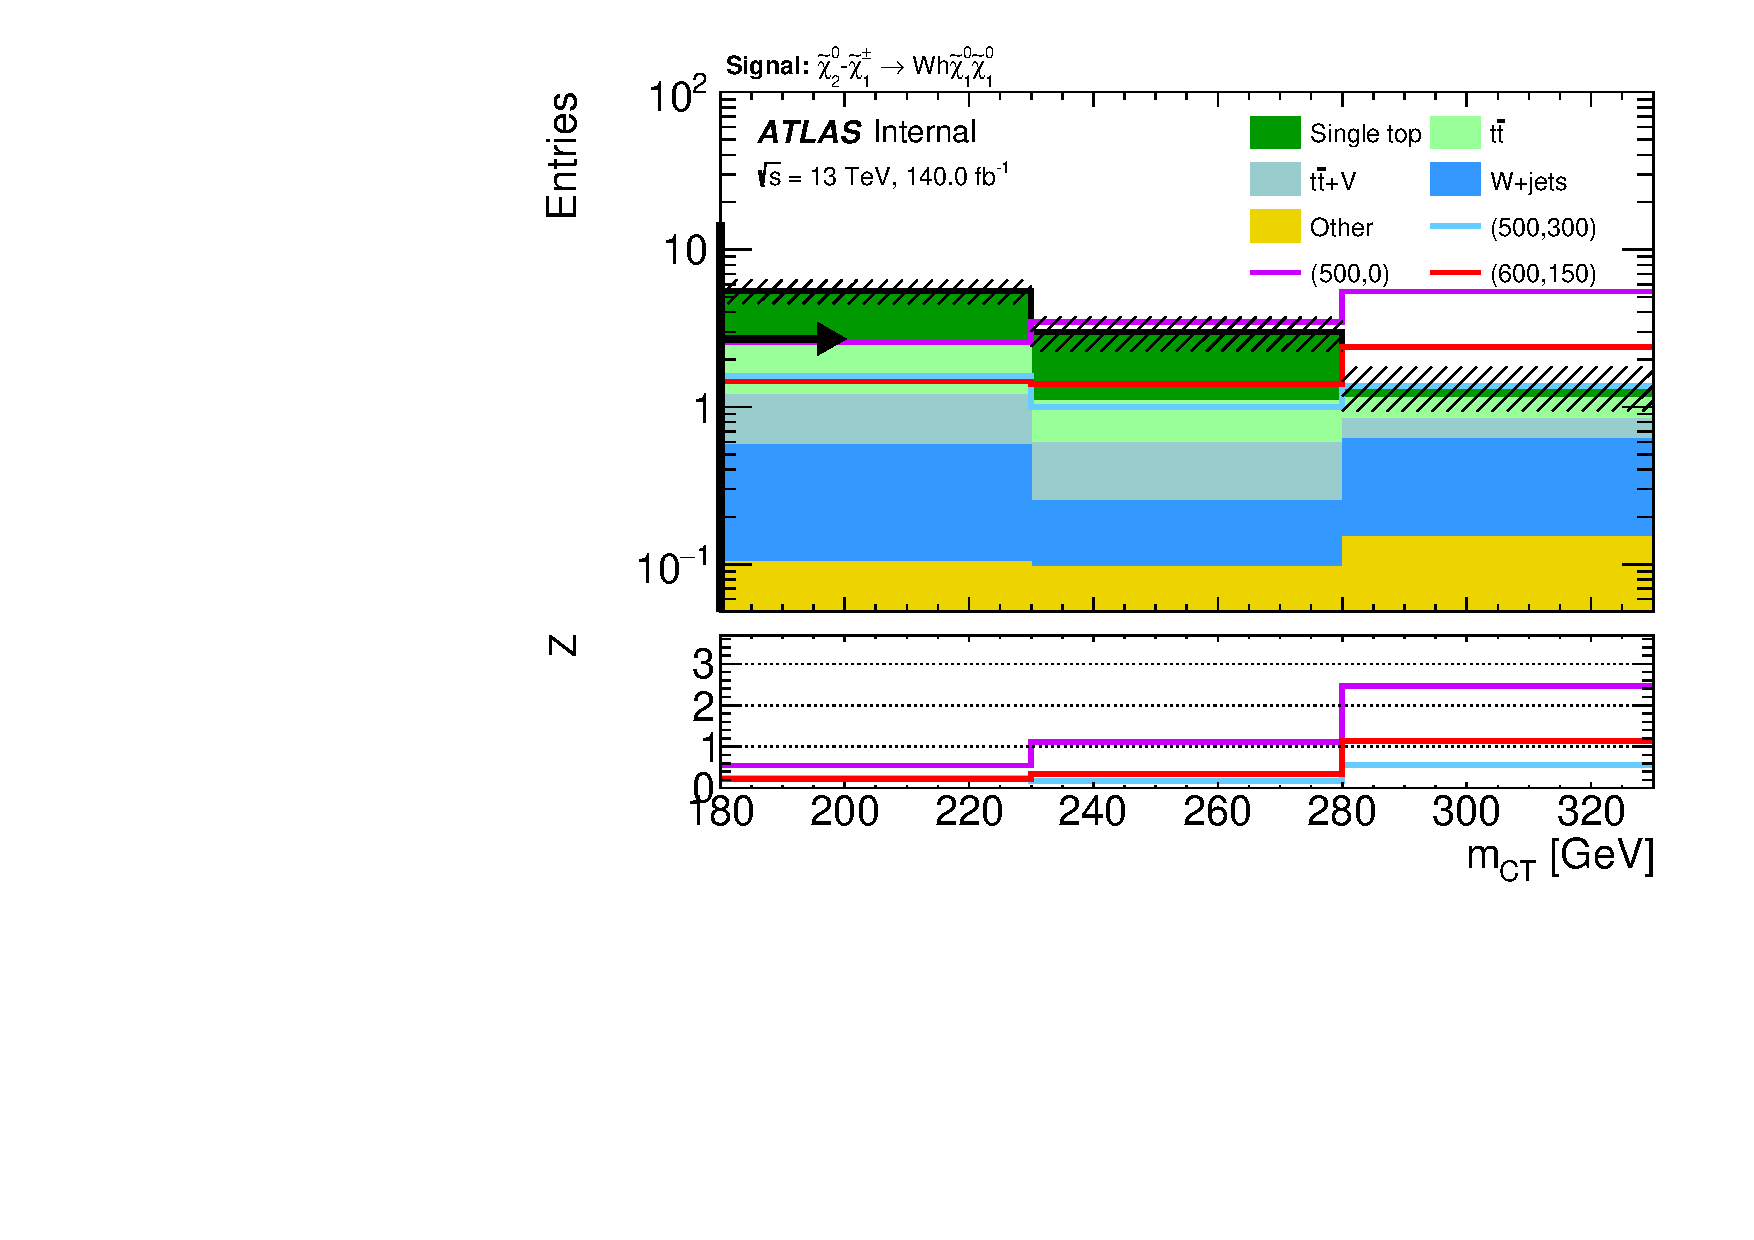
\includegraphics[width=\textwidth]{n1_SRMM_mct_bins/mct.pdf}
		\caption{\label{fig:Wh_reopt_second_round_n1_srmm_mct}}
	\end{subfigure}
	\begin{subfigure}[b]{0.4\linewidth}
		\centering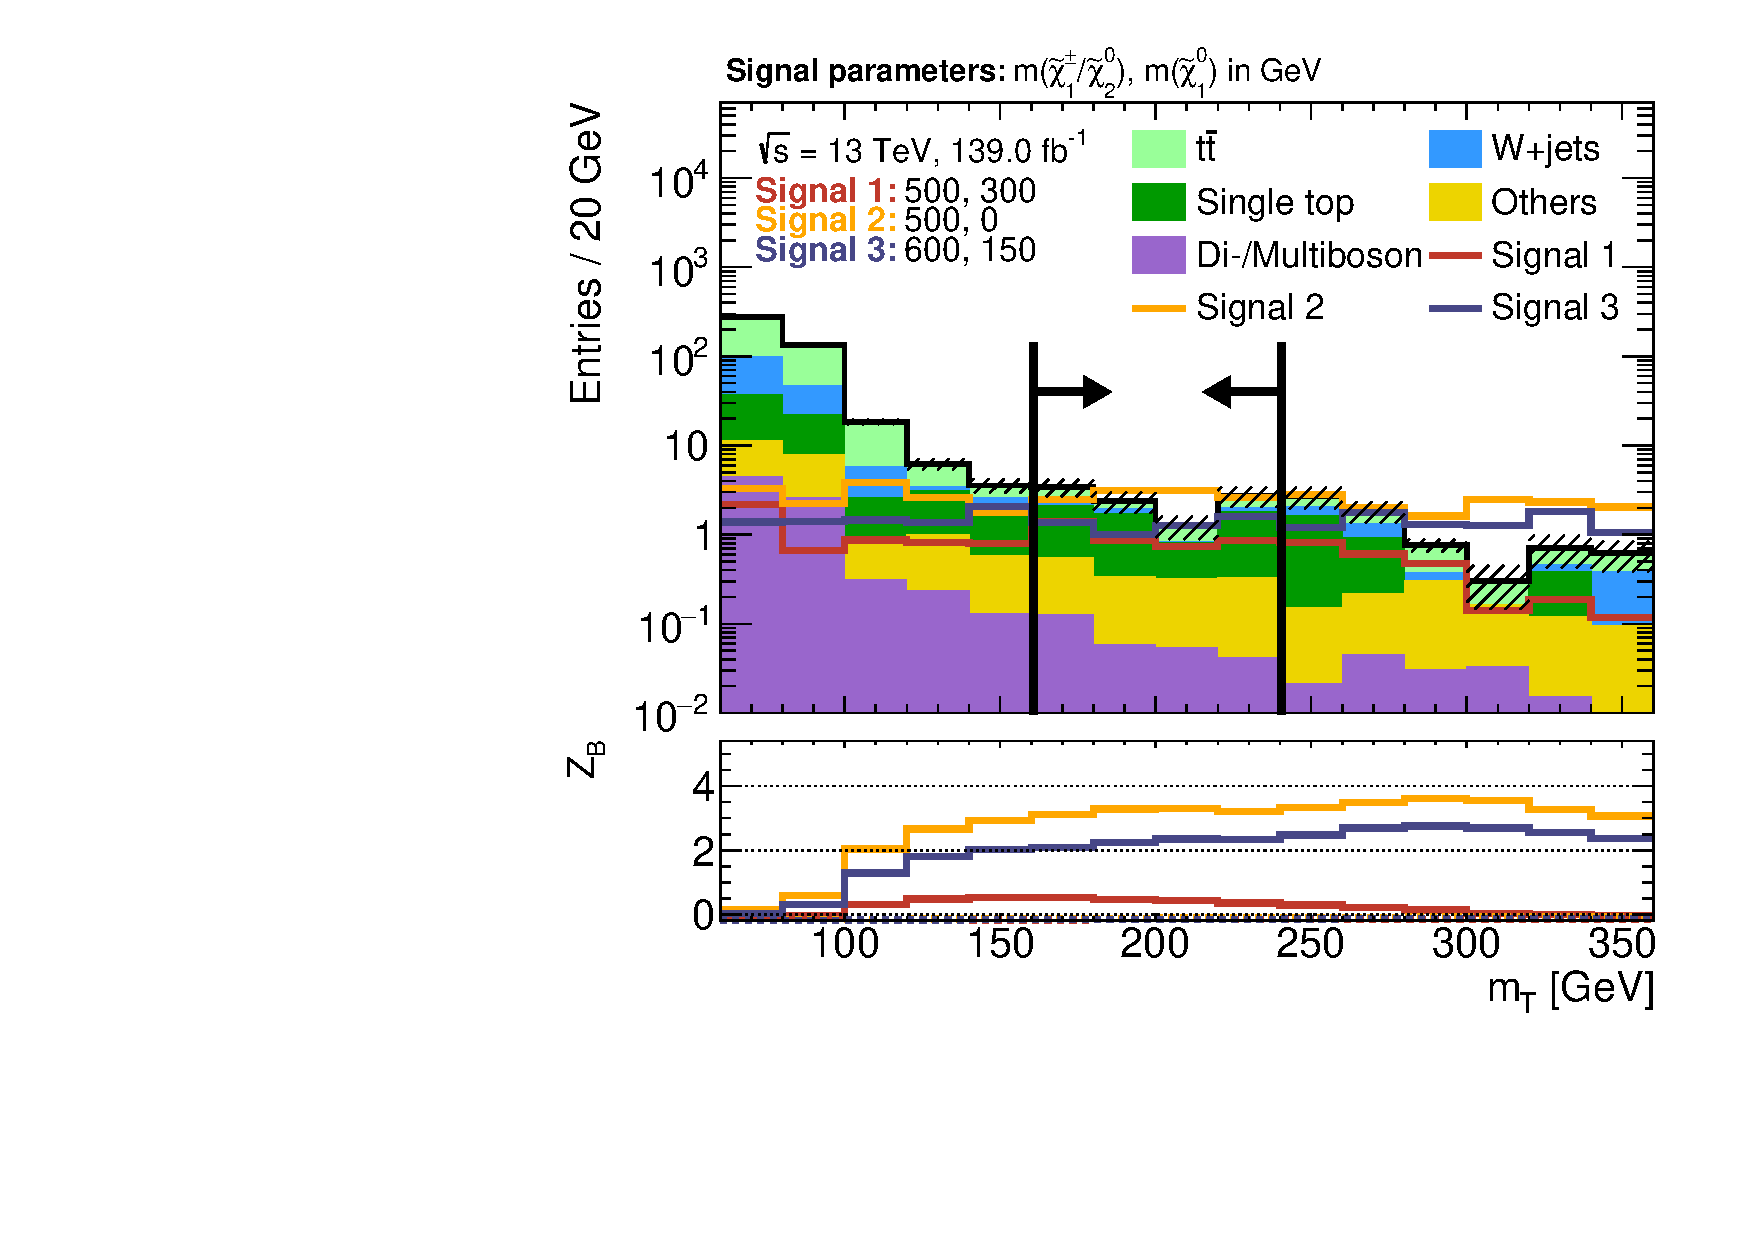
\includegraphics[width=\textwidth]{n1_SRMM_mct_bins/mt_both.pdf}
		\caption{\label{fig:Wh_reopt_second_round_n1_srmm_mt}}
	\end{subfigure}%
	\begin{subfigure}[b]{0.4\linewidth}
		\centering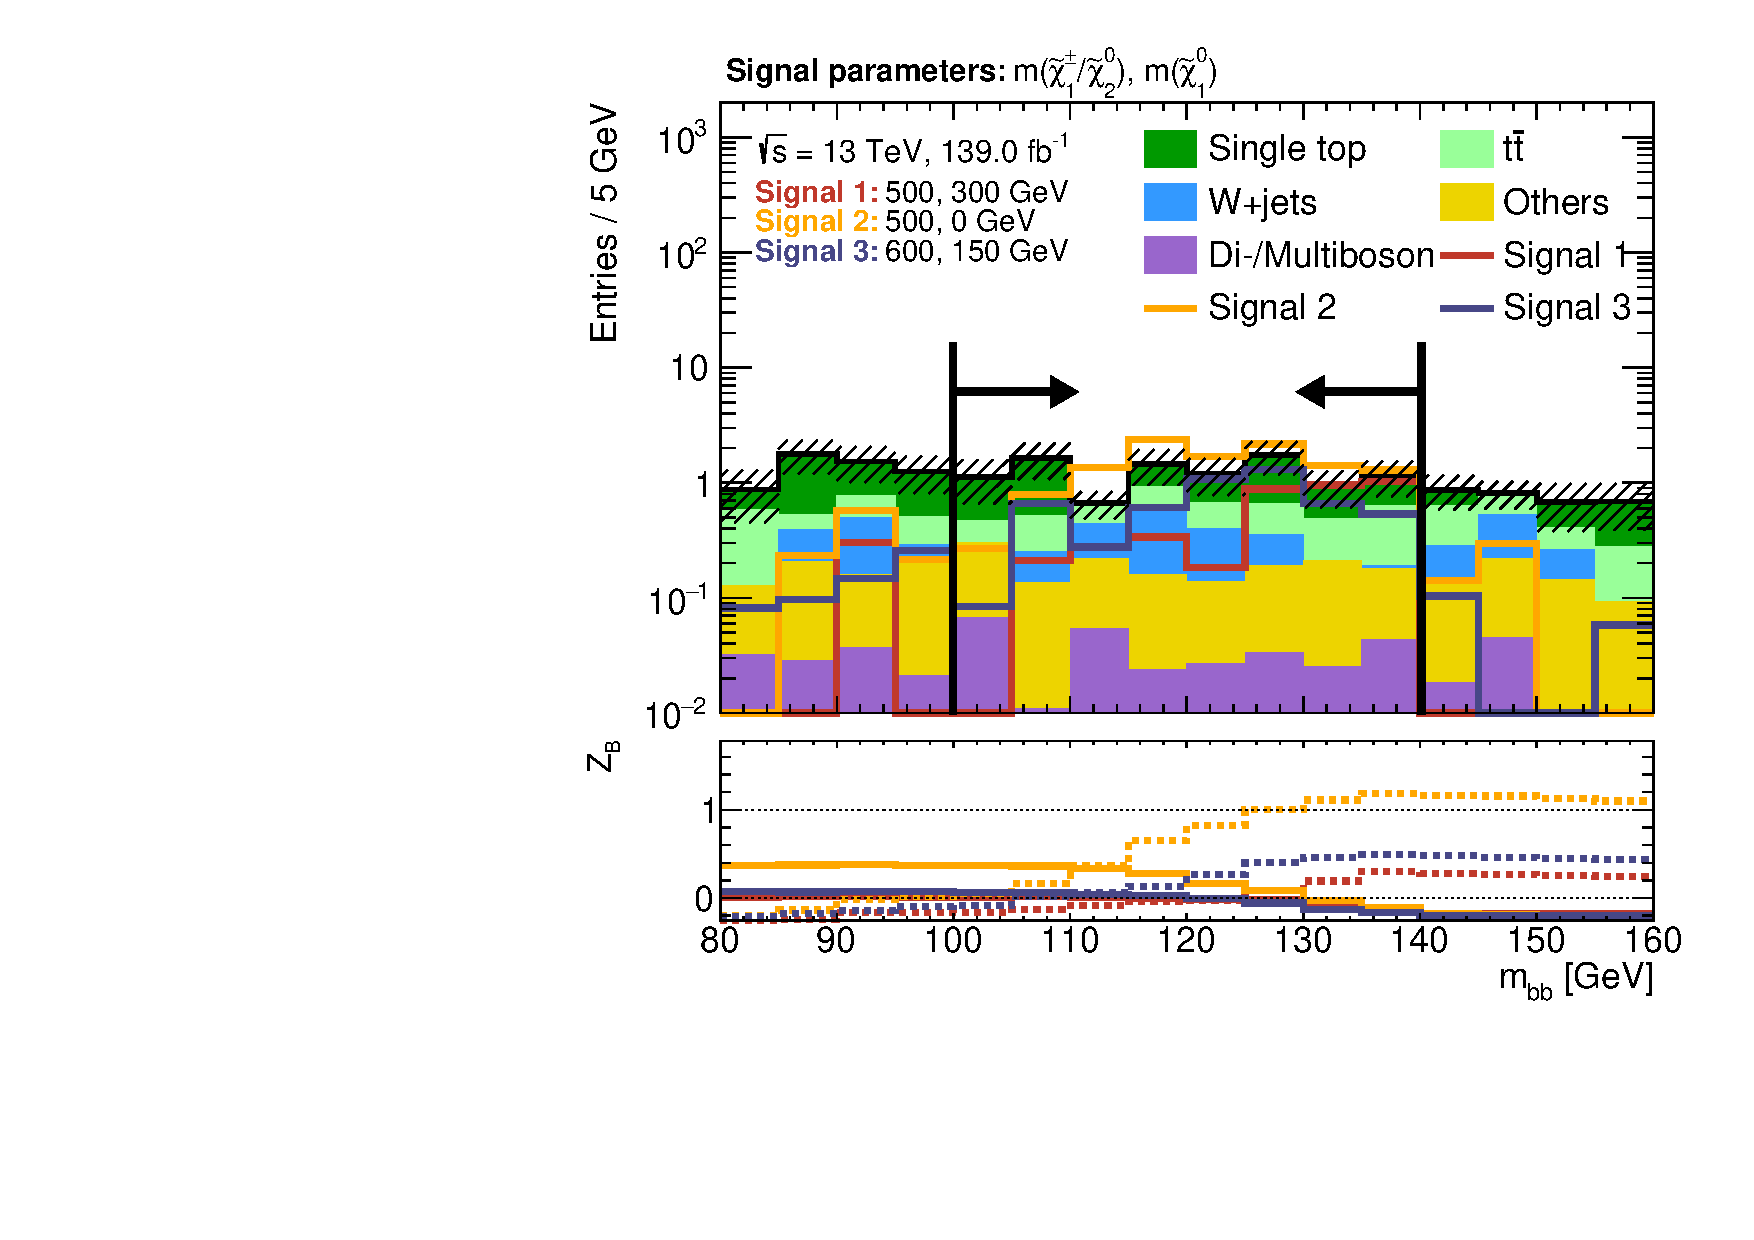
\includegraphics[width=\textwidth]{n1_SRMM_mct_bins/mbb_both.pdf}
		\caption{\label{fig:Wh_reopt_second_round_n1_srmm_mbb}}
	\end{subfigure}
%	\begin{subfigure}[b]{0.4\linewidth}
%		\centering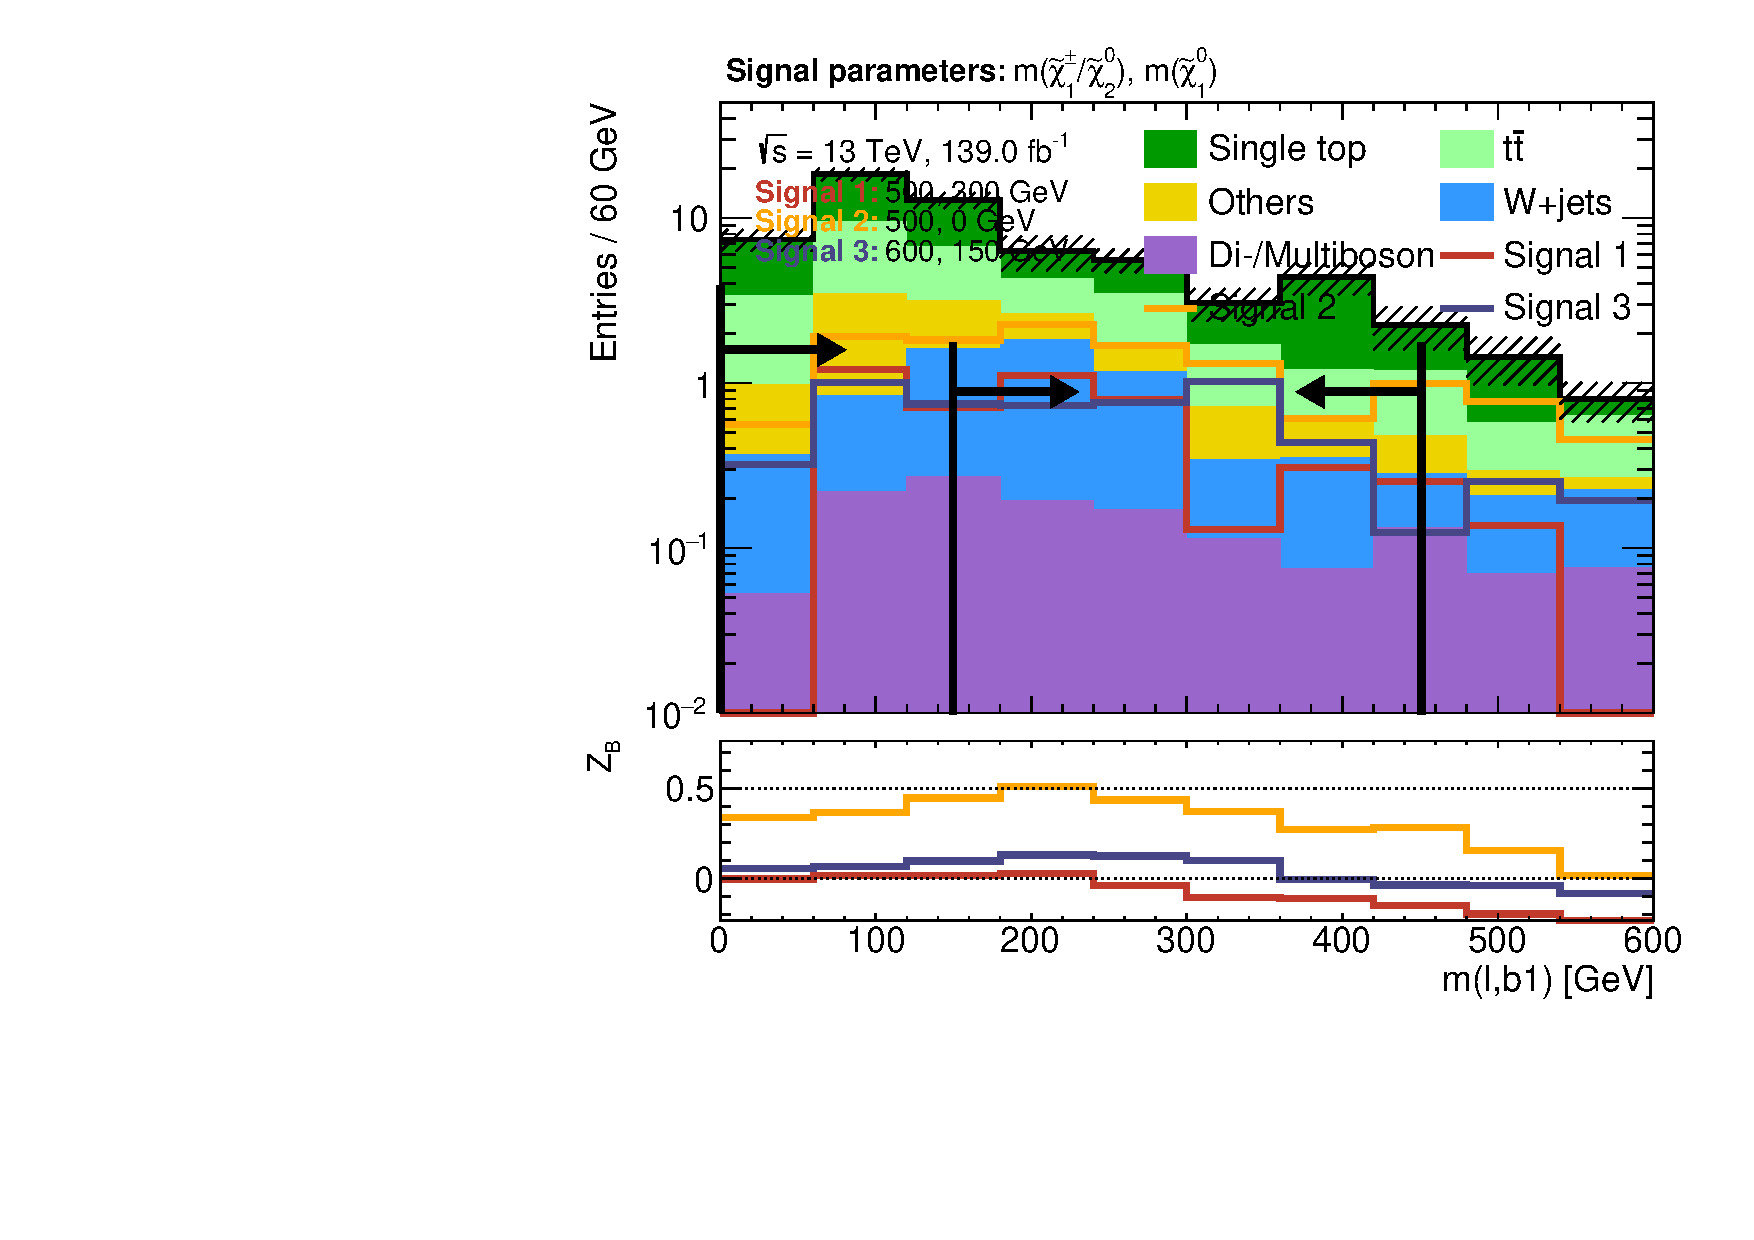
\includegraphics[width=\textwidth]{n1_SRMM_mct_bins/mlb1.pdf}
%		\caption{\label{fig:Wh_reopt_second_round_n1_srmm_mlb1}}
%	\end{subfigure}%
	\begin{subfigure}[b]{0.4\linewidth}
		\centering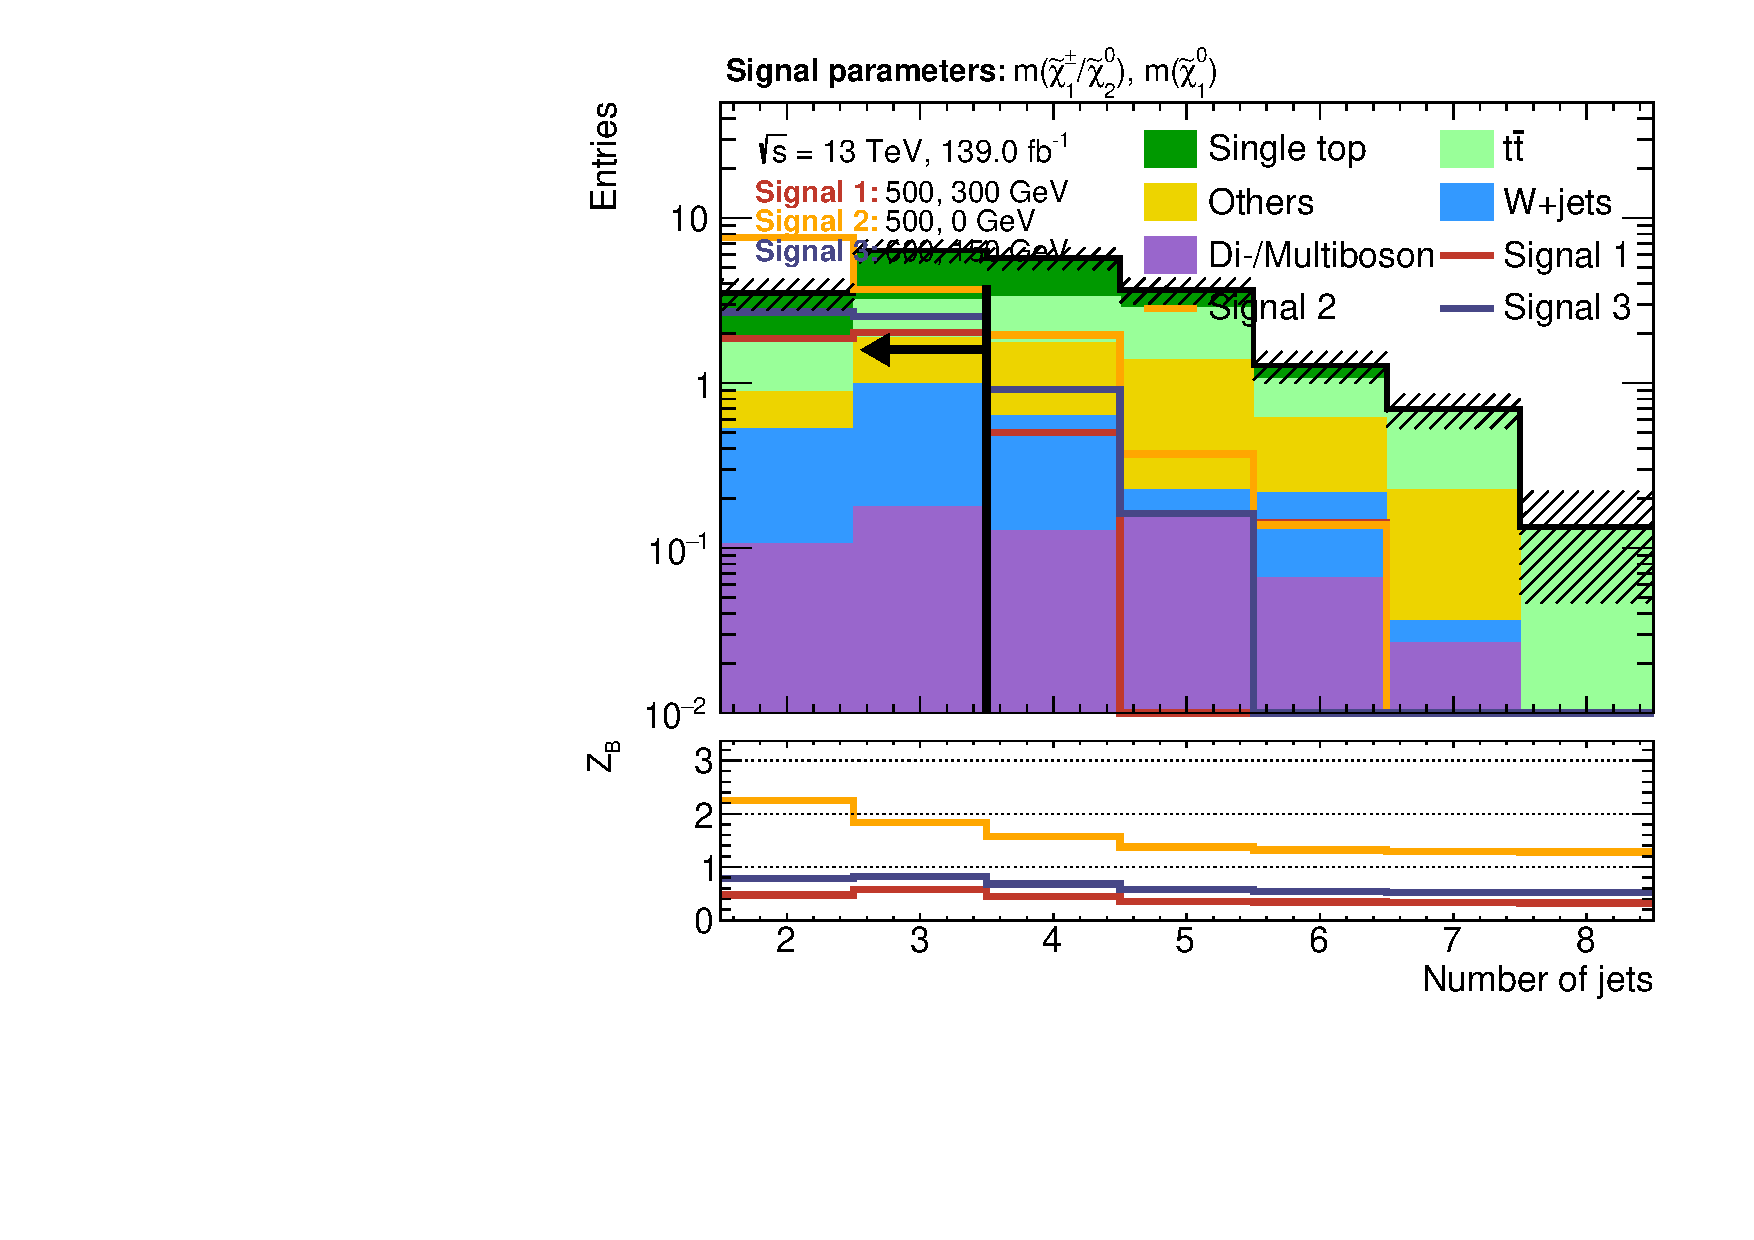
\includegraphics[width=\textwidth]{n1_SRMM_mct_bins/nJet30.pdf}
		\caption{\label{fig:Wh_reopt_second_round_n1_srmm_njet}}
	\end{subfigure}
	\caption{$N-1$ plots for SRMM, with exemplary signal points and all $\mct$ bins included. The dashed area represents \gls{mc} statistical uncertainty on the background. In all figures except \figname~\subref{fig:Wh_reopt_second_round_n1_srmm_mct}, the significance in the lower pad is obtained by summing up all the events in the direction of the cut arrow and includes 30\% uncertainty as well as MC statistical uncertainty. In \figname~\subref{fig:Wh_reopt_second_round_n1_srmm_mct} the significance is only computed on a bin-by-bin basis, \ie not summing up all events in the direction of the cut arrow.}
	\label{fig:Wh_reopt_second_round_n1_srmm}
\end{figure}

\begin{figure}
	\centering
	\begin{subfigure}[b]{0.4\linewidth}
		\centering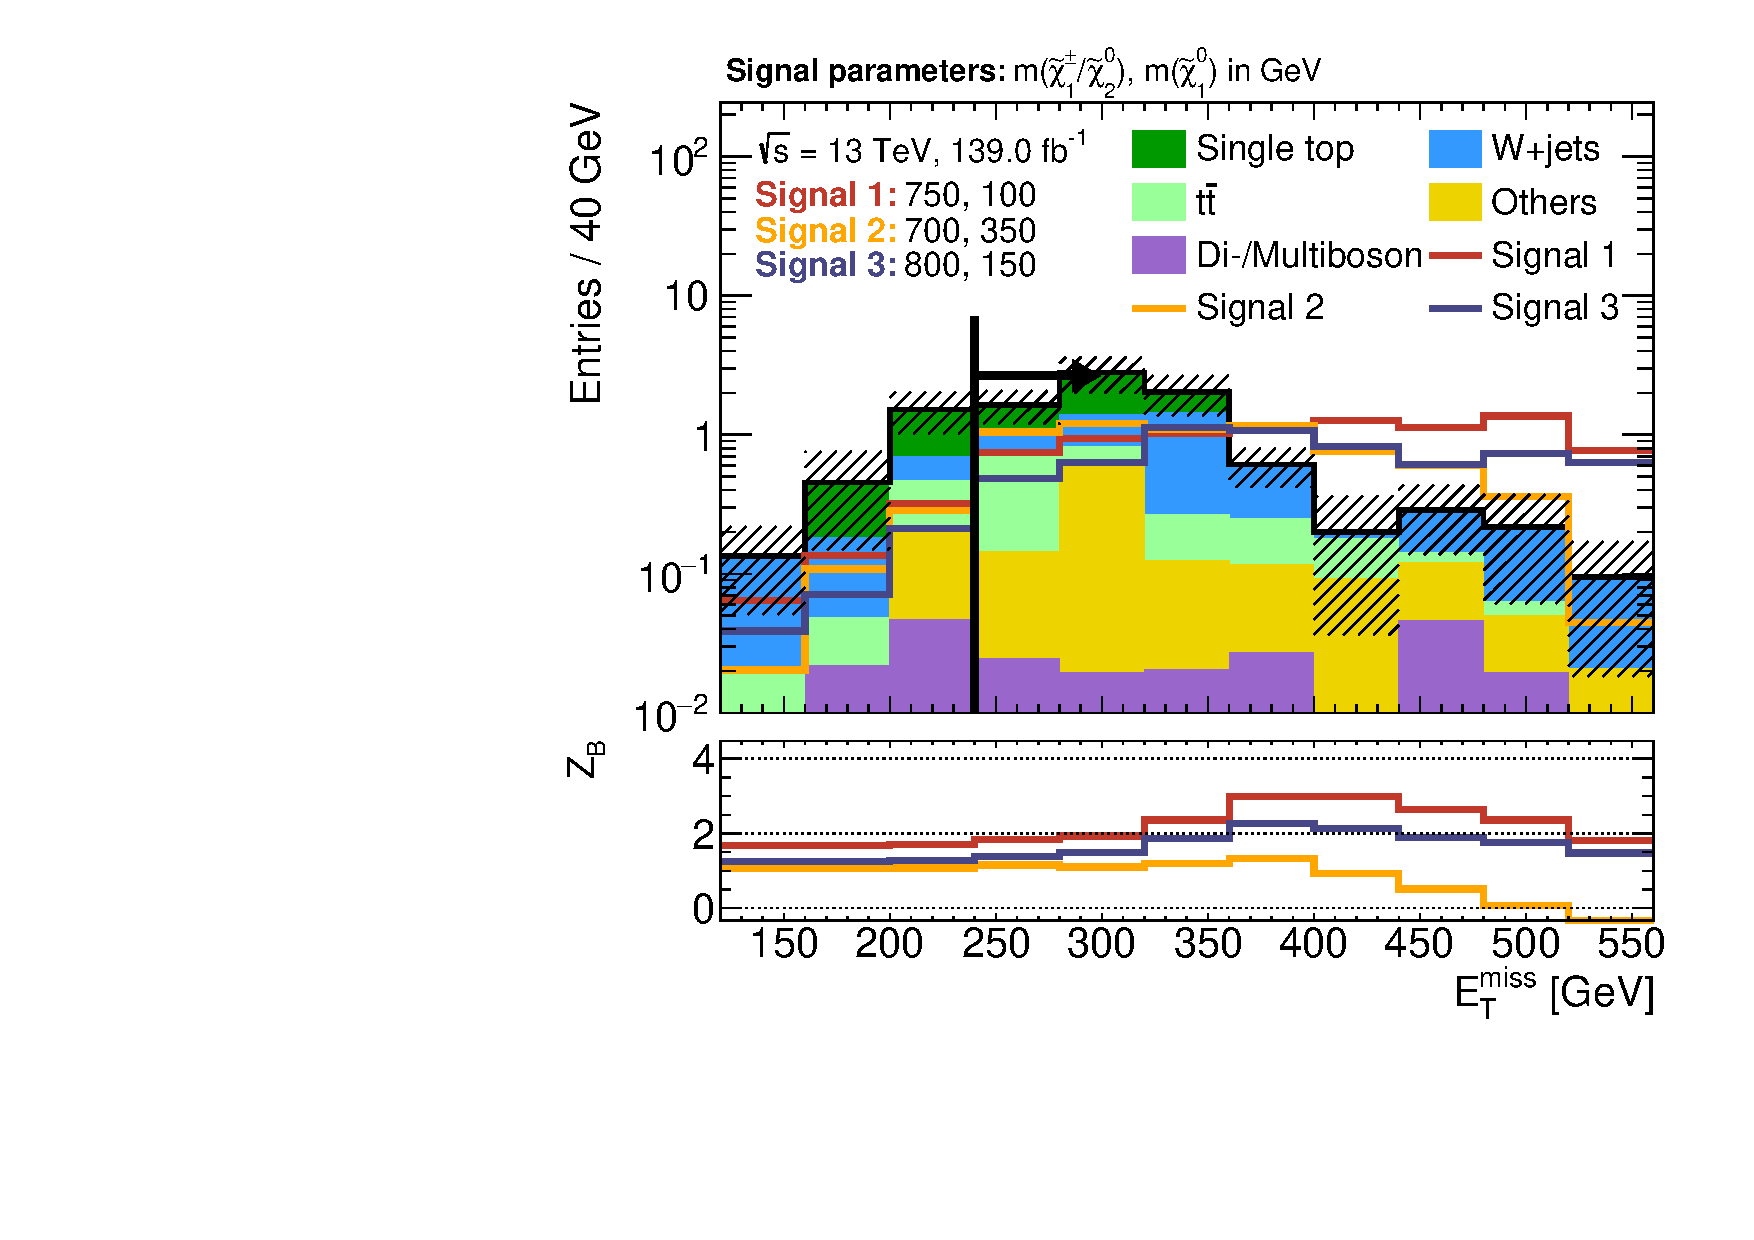
\includegraphics[width=\textwidth]{n1_SRHM_mct_bins/met.pdf}
		\caption{\label{fig:Wh_reopt_second_round_n1_srhm_met}}
	\end{subfigure}%
	\begin{subfigure}[b]{0.4\linewidth}
		\centering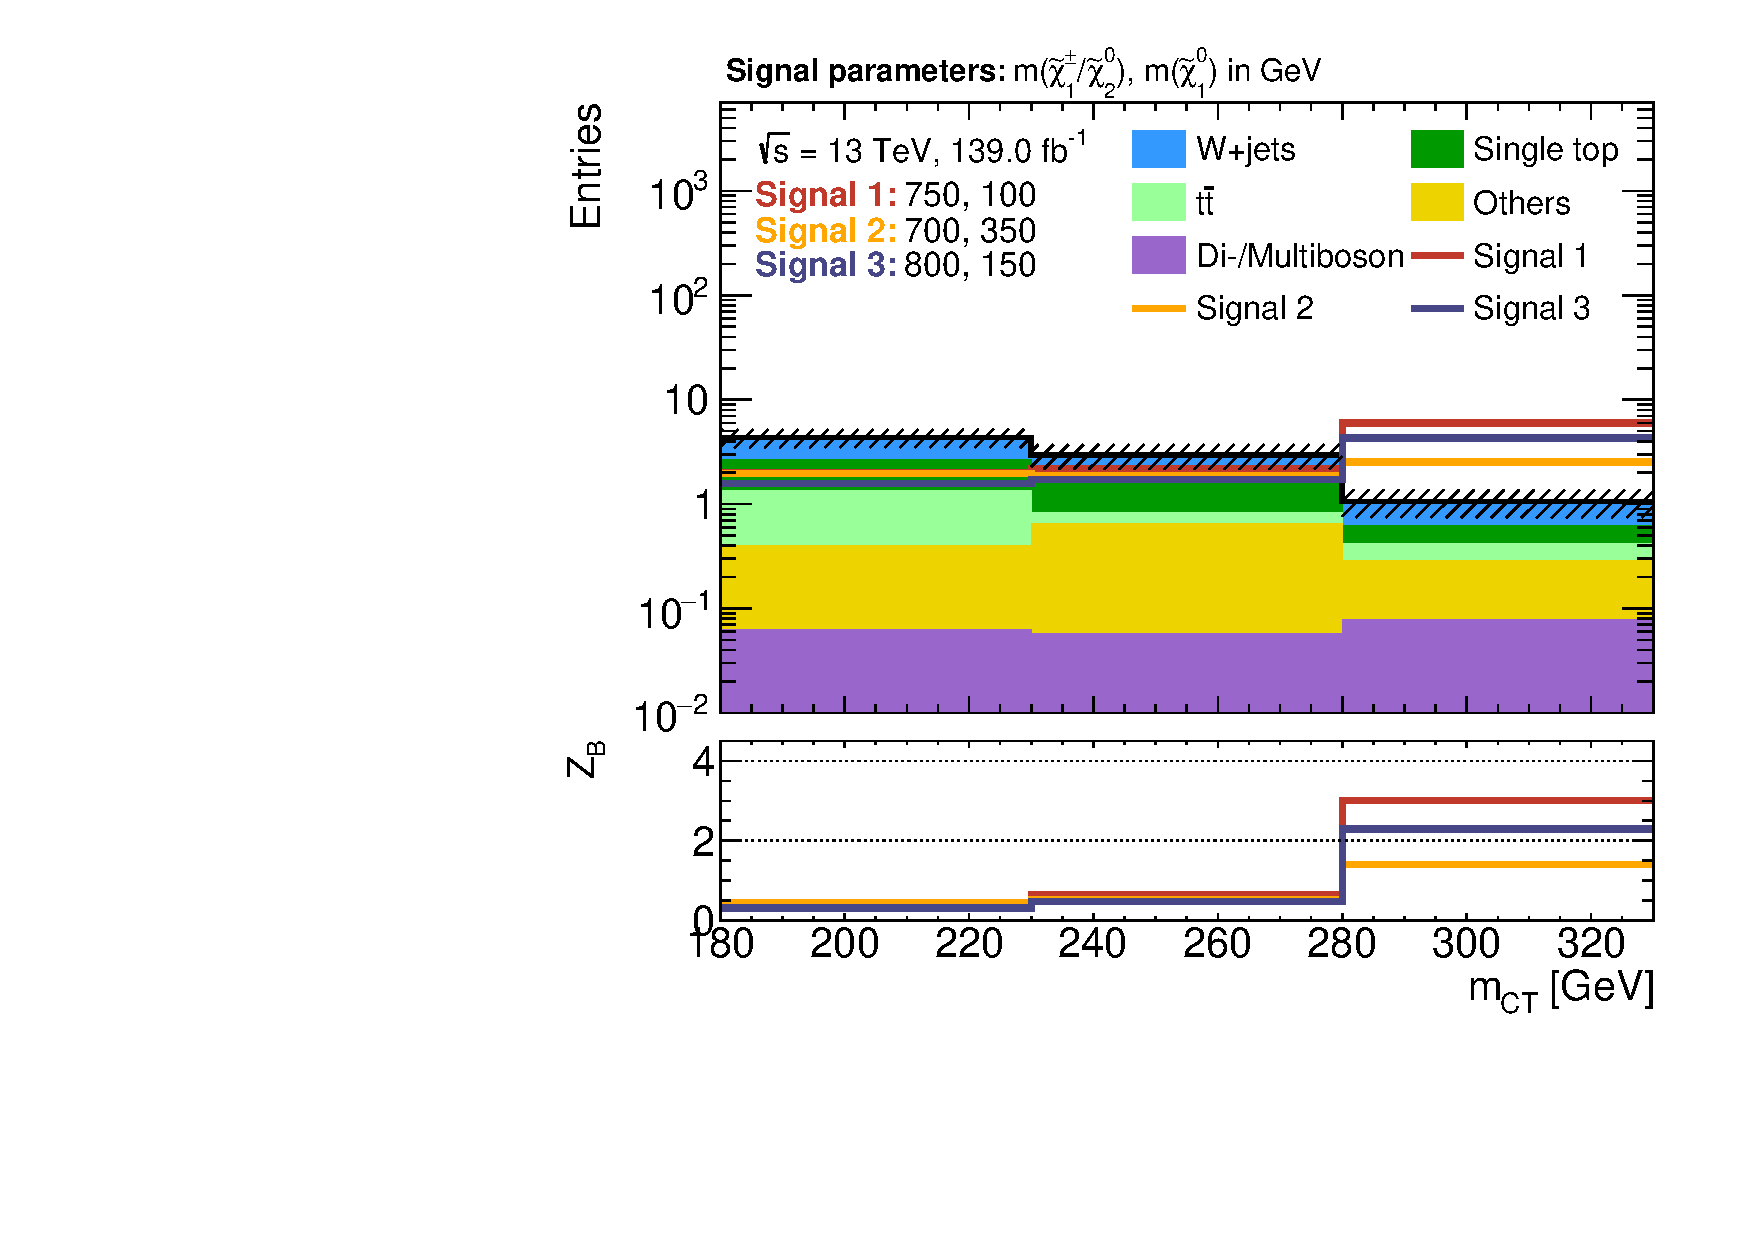
\includegraphics[width=\textwidth]{n1_SRHM_mct_bins/mct.pdf}
		\caption{\label{fig:Wh_reopt_second_round_n1_srhm_mct}}
	\end{subfigure}
	\begin{subfigure}[b]{0.4\linewidth}
		\centering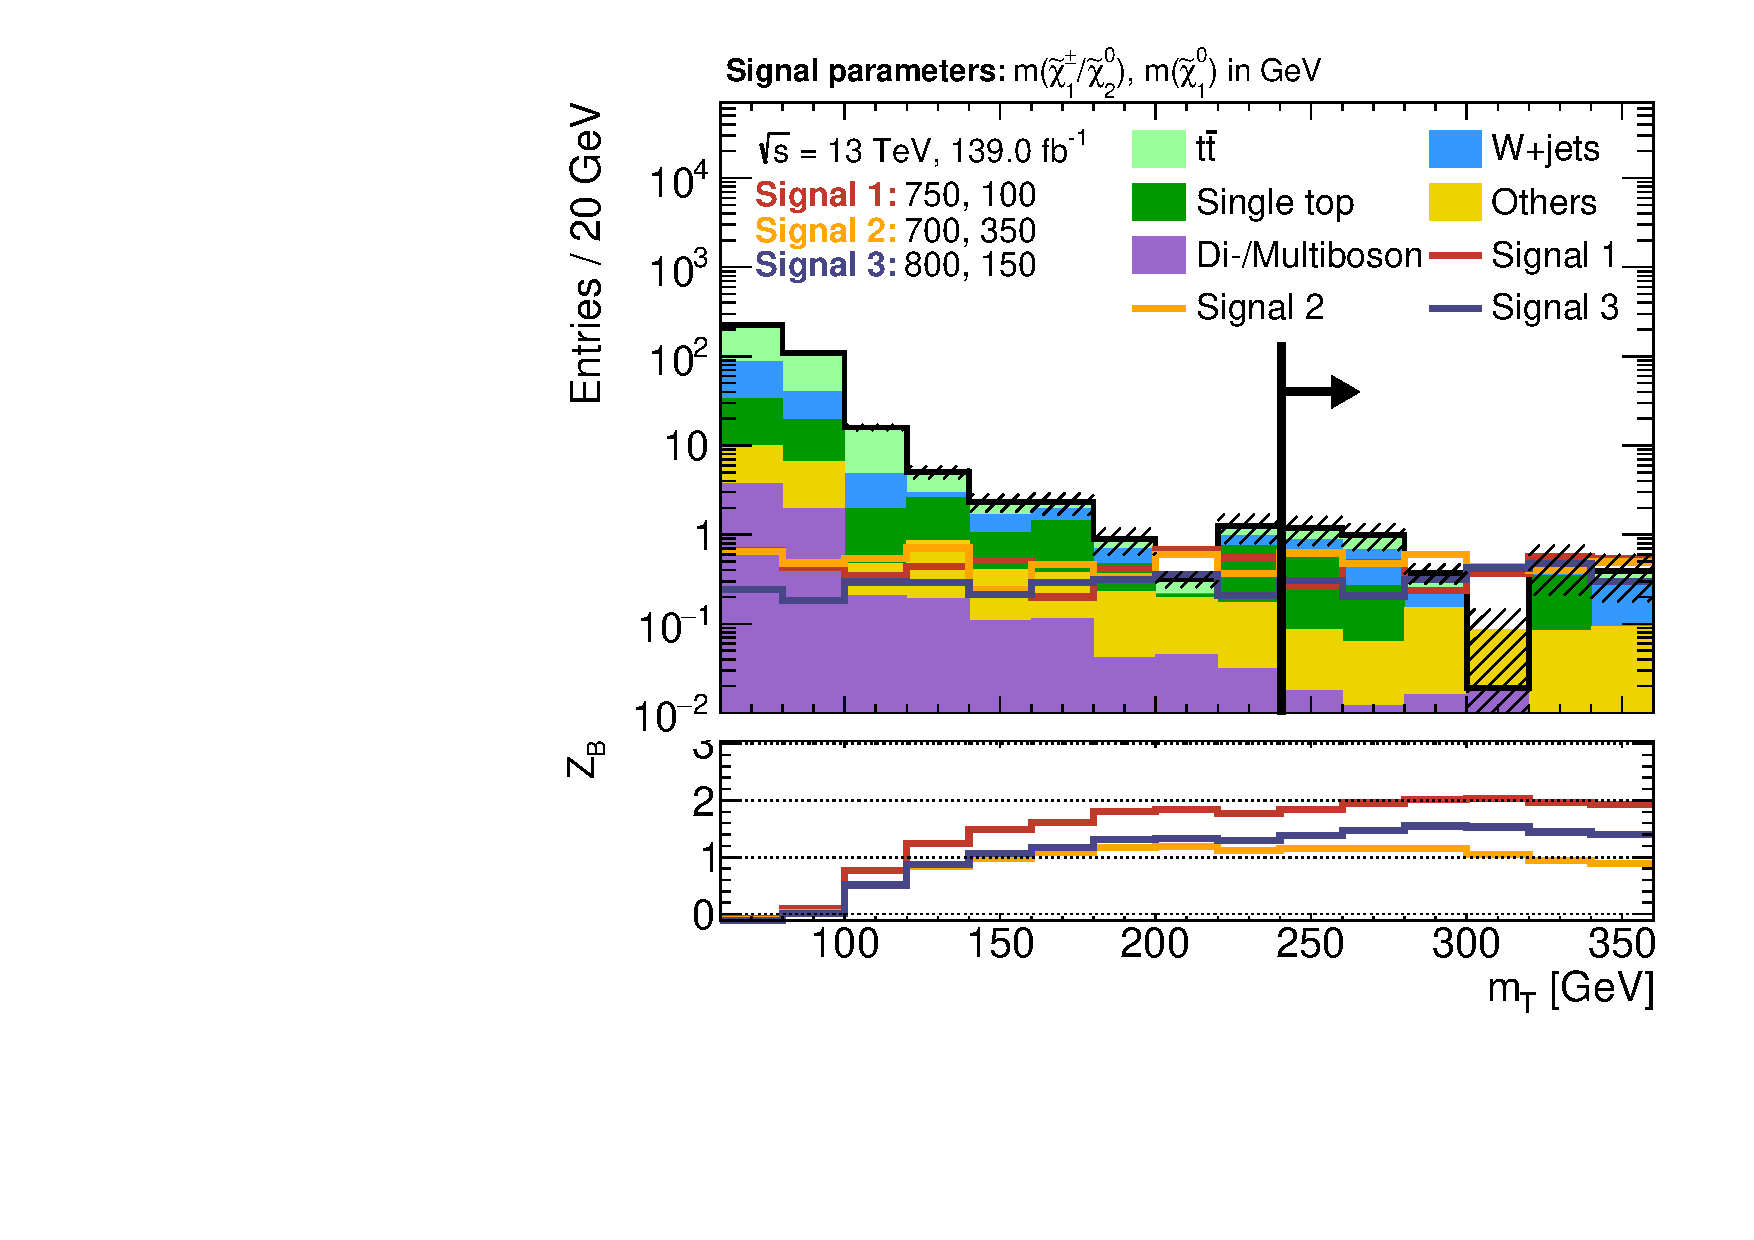
\includegraphics[width=\textwidth]{n1_SRHM_mct_bins/mt_both.pdf}
		\caption{\label{fig:Wh_reopt_second_round_n1_srhm_mt}}
	\end{subfigure}%
	\begin{subfigure}[b]{0.4\linewidth}
		\centering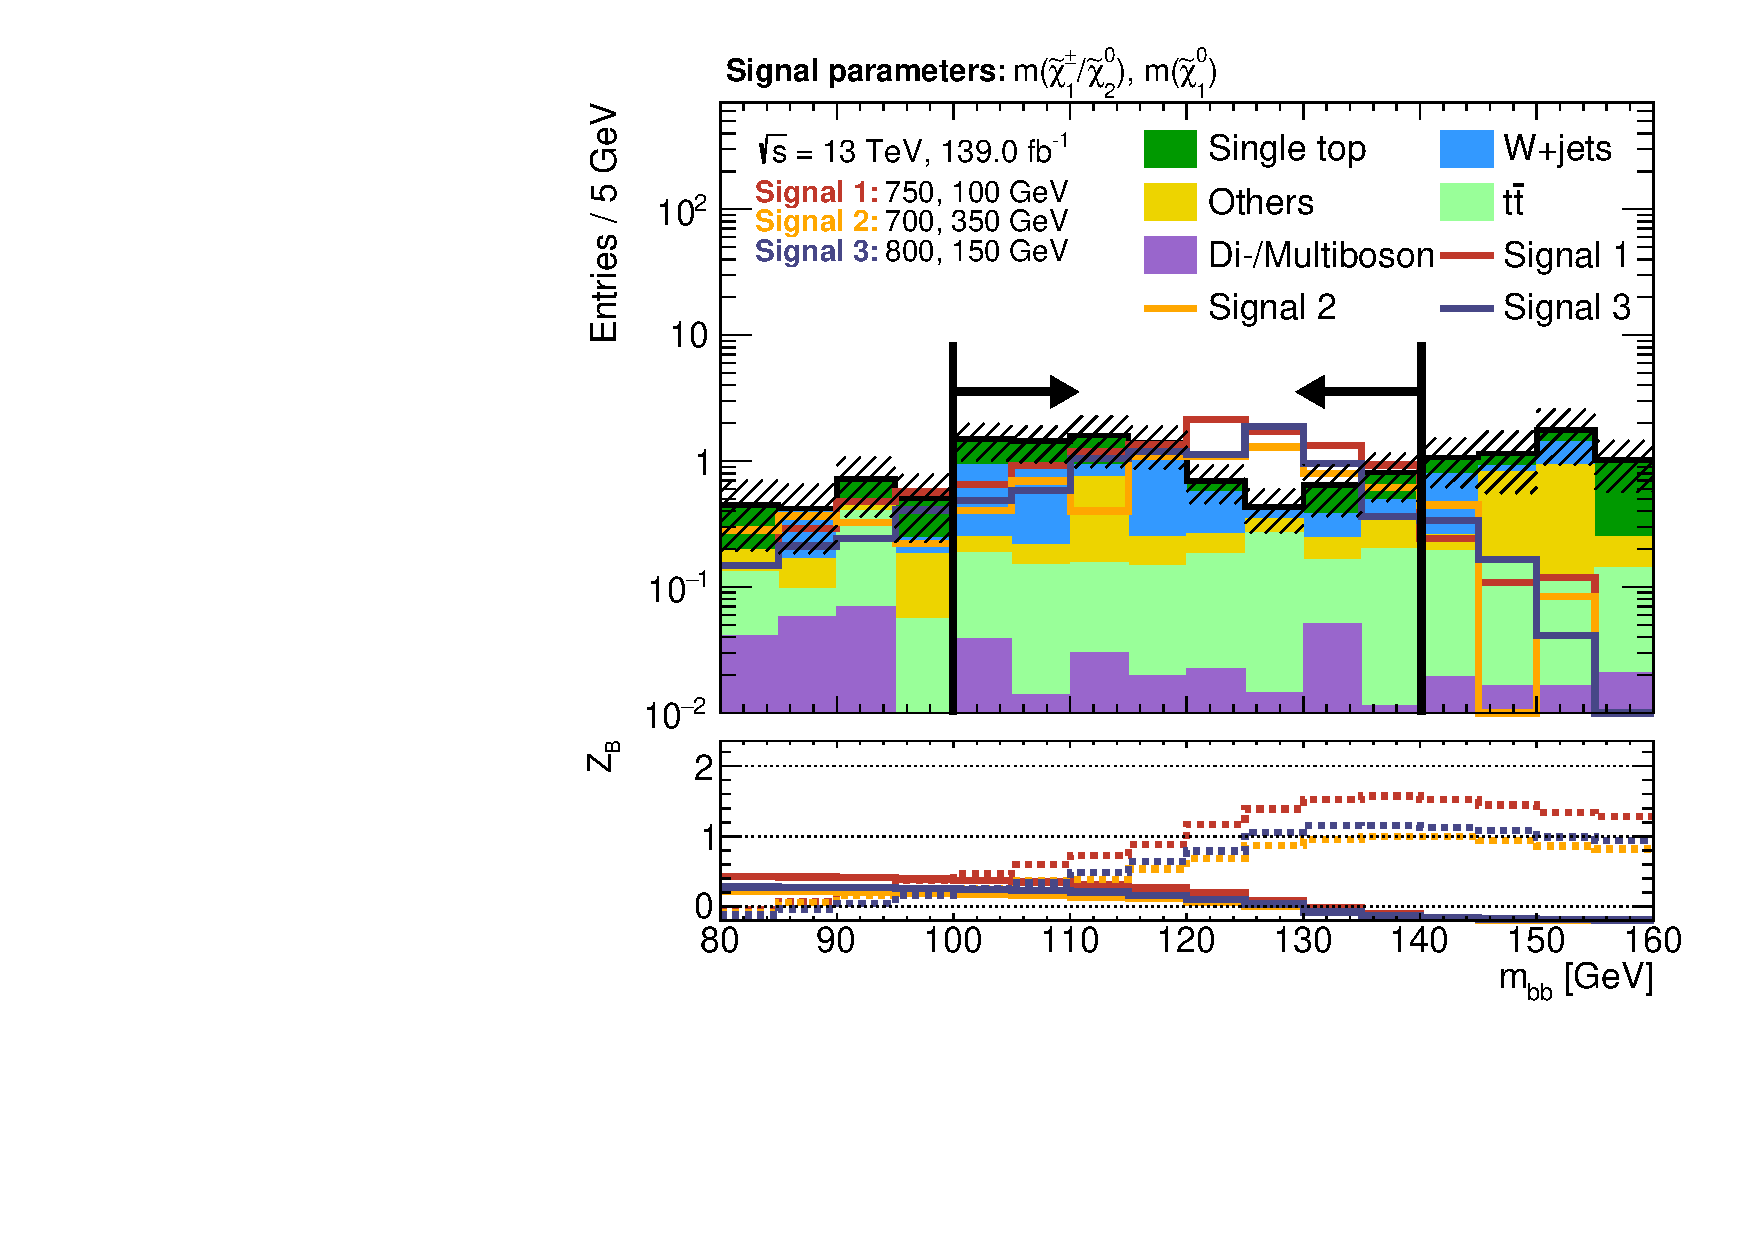
\includegraphics[width=\textwidth]{n1_SRHM_mct_bins/mbb_both.pdf}
		\caption{\label{fig:Wh_reopt_second_round_n1_srhm_mbb}}
	\end{subfigure}
	\begin{subfigure}[b]{0.4\linewidth}
		\centering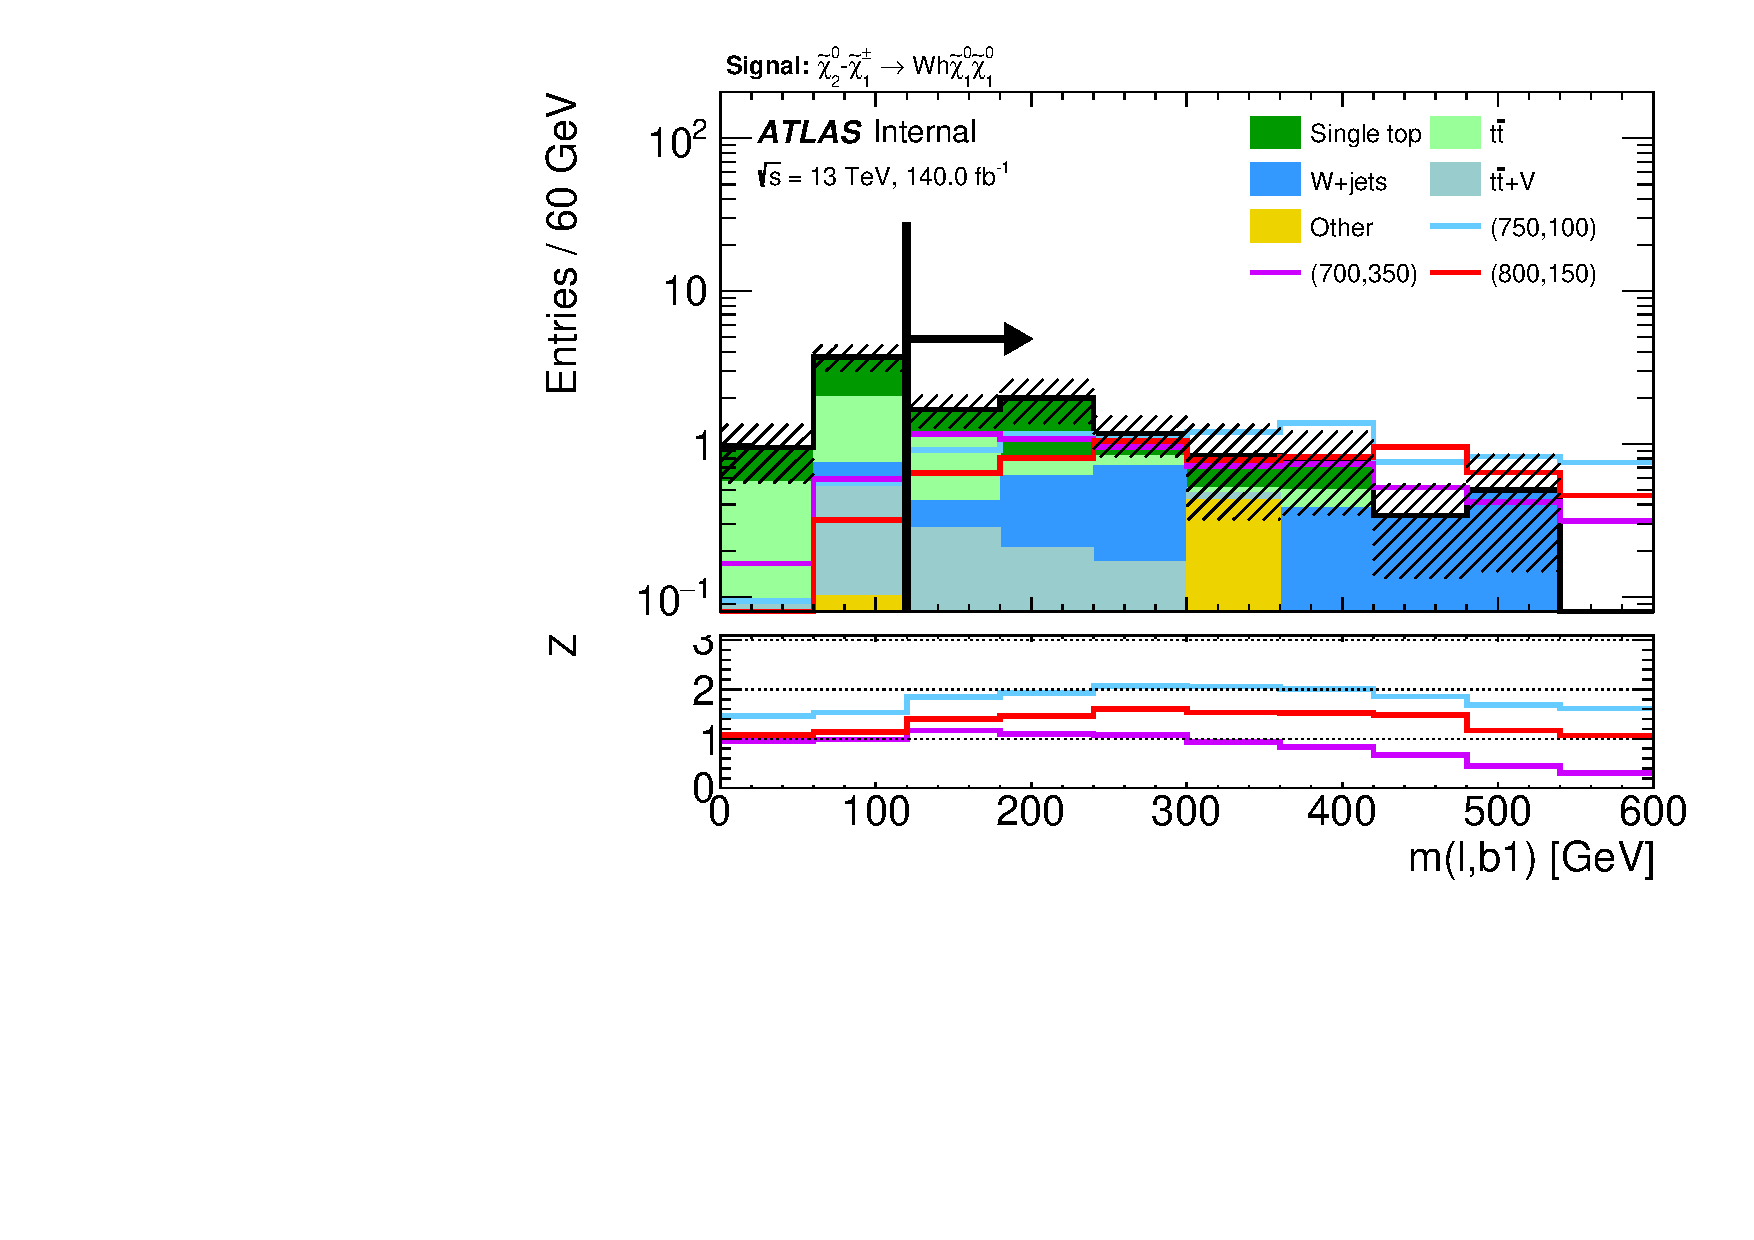
\includegraphics[width=\textwidth]{n1_SRHM_mct_bins/mlb1.pdf}
		\caption{\label{fig:Wh_reopt_second_round_n1_srhm_mlb1}}
	\end{subfigure}%
	\begin{subfigure}[b]{0.4\linewidth}
		\centering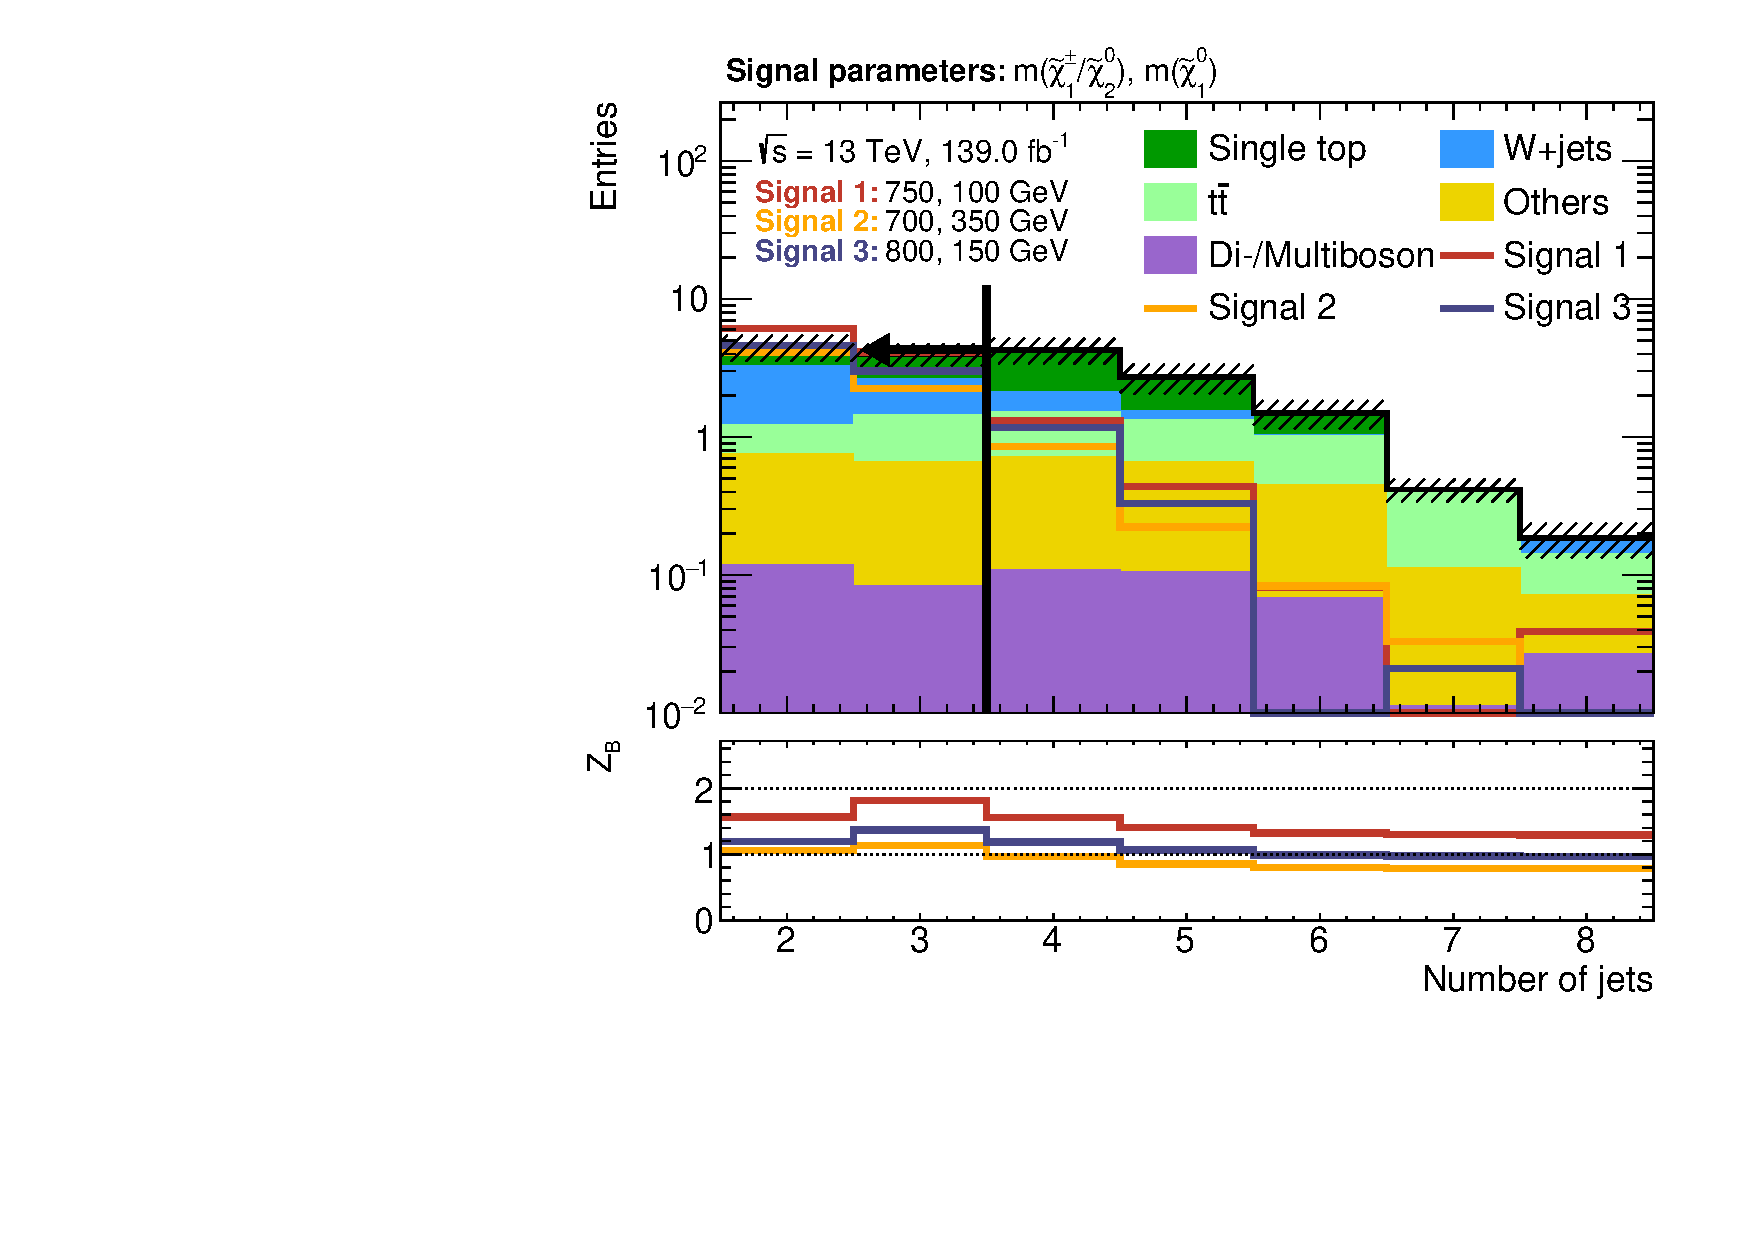
\includegraphics[width=\textwidth]{n1_SRHM_mct_bins/nJet30.pdf}
		\caption{\label{fig:Wh_reopt_second_round_n1_srhm_njet}}
	\end{subfigure}
	\caption{$N-1$ plots for SRHM, with exemplary signal points and all $\mct$ bins included. The dashed area represents \gls{mc} statistical uncertainty on the background. In all figures except \figname~\subref{fig:Wh_reopt_second_round_n1_srhm_mct}, the significance in the lower pad is obtained by summing up all the events in the direction of the cut arrow and includes 30\% uncertainty as well as MC statistical uncertainty. In \figname~\subref{fig:Wh_reopt_second_round_n1_srhm_mct} the significance is only computed on a bin-by-bin basis, \ie not summing up all events in the direction of the cut arrow.}
	\label{fig:Wh_reopt_second_round_n1_srhm}
\end{figure}




